\section{Numerical results}
\label{sec:results}

\subsection{Parameter distribution}
\label{sec:param_sampling}

Applying the methodology described in Section~\ref{sec:param_dist_fit}, $S=919$ parameter samples are drawn and \eqref{caboodle} is solved for each sample with no stimulus applied. Of these 919 runs, 670 of them fail due to ode15s terminating prematurely because its time steps became too small. The remaining 249 yields 139 solutions for which the radius reaches a stable steady state (at least for the duration of the time integration) and 110 solutions for which the radius reaches a steady state but subsequently becomes transient. The left panel of Figure~\ref{steady_states} displays four representative solutions for the radius; the red curves remain in steady state for the duration of our time integration whereas the black curves revert into a transit regime after some time in or near steady state. The right panel of Figure~\ref{steady_states} displays the samples for two parameters (defined in the buffer equation \eqref{eqn:buff}, see the Supplementary Material for details) which are found to be highly influential in determining the behavior of the solution. A blue \textcolor{blue}{*} indicates a sample where the solver terminated prematurely, a yellow \textcolor{yellow}{$\Diamond$} indicates a sample where an unstable steady state was observed, a red \textcolor{red}{$\circ$} indicates a sample where the solution remained in steady state. A strong correlation determining the behavior of the solution is observed. The two parameters in question, denoted by ($\theta_{120},\theta_{121}$), occur in the buffer equation defined by
\begin{eqnarray}\label{eqn:buff}
[K^+]_e+B \quad\begin{array}{c}
f_f =\frac{\theta_{118}}{1+exp(\frac{-[K^+]_e+\theta_{120}}{\theta_{121}})}\\ 
 \rightleftharpoons \\
f_r=\theta_{118}
\end{array} 
[K^+]_b \nonumber \\
\frac{d[K^+]_b}{dt}=f_f[K^+]_e(\theta_{119}-[K^+]_b)-f_r[K^+]_b \nonumber \\
\end{eqnarray}
The parameters $\theta_{120}$ and $\theta_{121}$ have values 5.5 and 1.09, representing a shift and scaling in the forward rate constant, respectively. 
\begin{figure}[h]
\centering
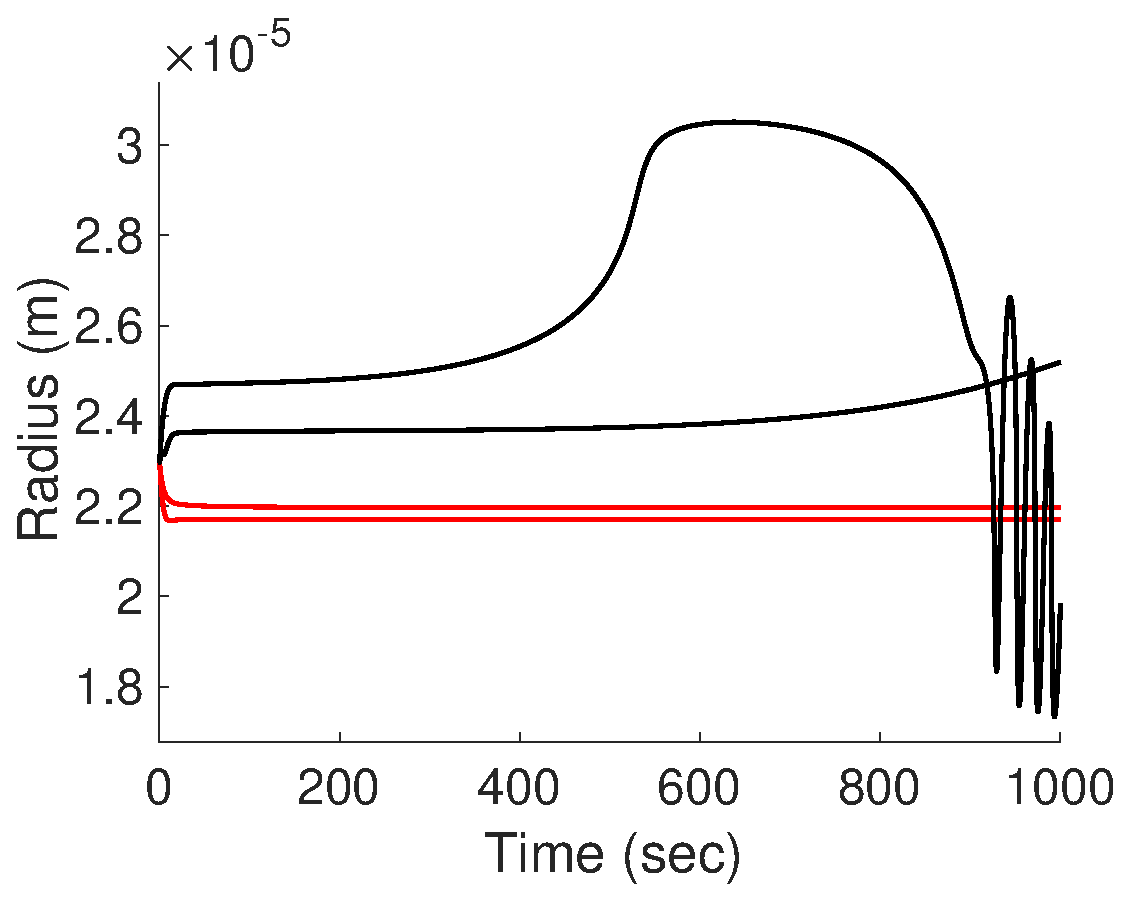
\includegraphics[width=.4 \textwidth]{Figures/Steady_State_Curves.eps}
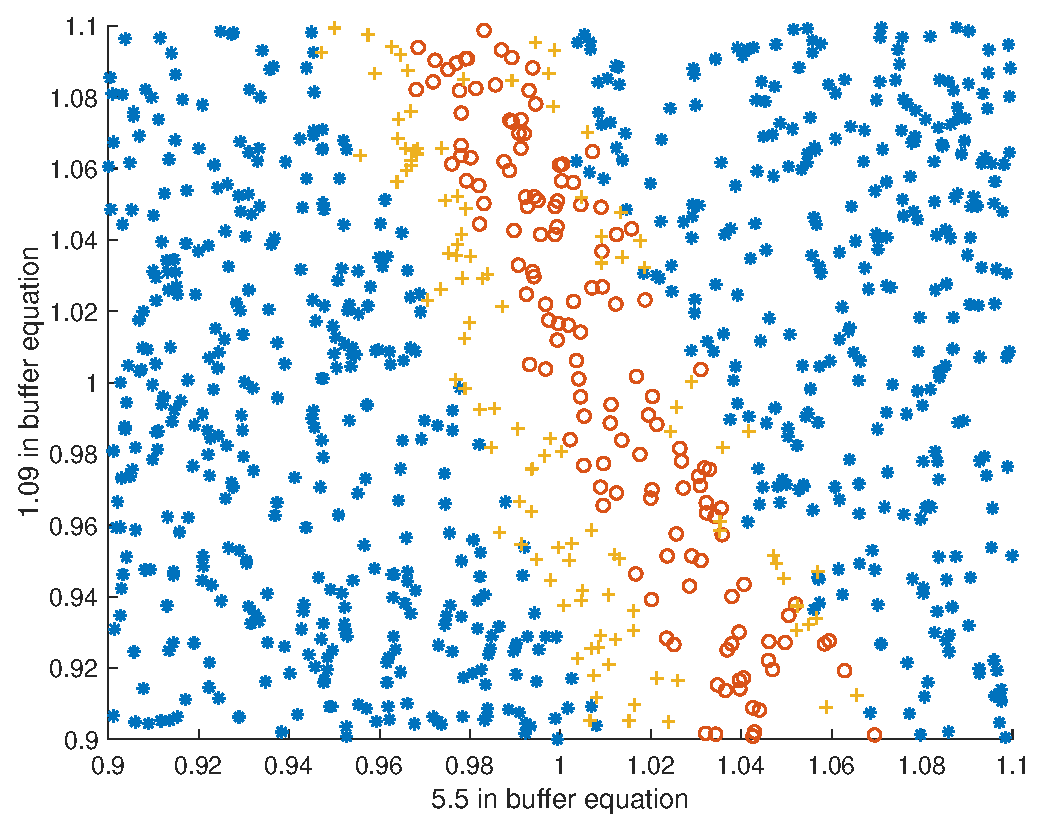
\includegraphics[width=.4 \textwidth]{Figures/First_Iteration_Samples.eps}
\caption{Left: examples of stable (red) and unstable (black) steady state solutions. Right: samples of the buffer parameters $(\theta_{120},\theta_{121})$ using uniform independent sampling. A blue \textcolor{blue}{*} indicates the sample yielded a premature termination of the solver, a yellow \textcolor{yellow}{$\Diamond$} indicates the sample yielded an unstable steady state, a red \textcolor{red}{$\circ$} indicates the sample yielded a stable steady state.}
\label{steady_states}
\end{figure}

Observing this correlation, we use the accepted samples to fit $(\theta_{120},\theta_{121})$ with a bivariate Frank copula with beta marginals. The experiment is repeated by sampling the two correlated parameters from this bivariate distribution and all other parameter from their original uniform distributions. After four iterations refining the joint distribution of $(\theta_{120},\theta_{121})$, we were able to generate 902 out of 960 samples which yielded solutions with stable steady states (51 solutions had unstable steady states and 7 had premature solver terminations). This fitted distribution is used for all subsequent analysis. 

Samples are drawn and the model, with a stimulus applied (in two separate cases, the 10 second rectangular pulse and the 16 second experimental pulse), is run for each sample. This results in solutions exhibiting three different physiological regimes; they are displayed in Figure~\ref{solution_regimes} where the radius is plotted as a function of time. The leftmost panel corresponds to the typical case when the radius increases in response to the stimulus and then decreases when it is removed; the center panel corresponds to an atypical case where the radius has an initial decrease in response to the stimulus; the right panel corresponds to another atypical case where the radius reaches another steady state and does not decrease after the stimulus is removed.

\begin{figure}[h]
\centering
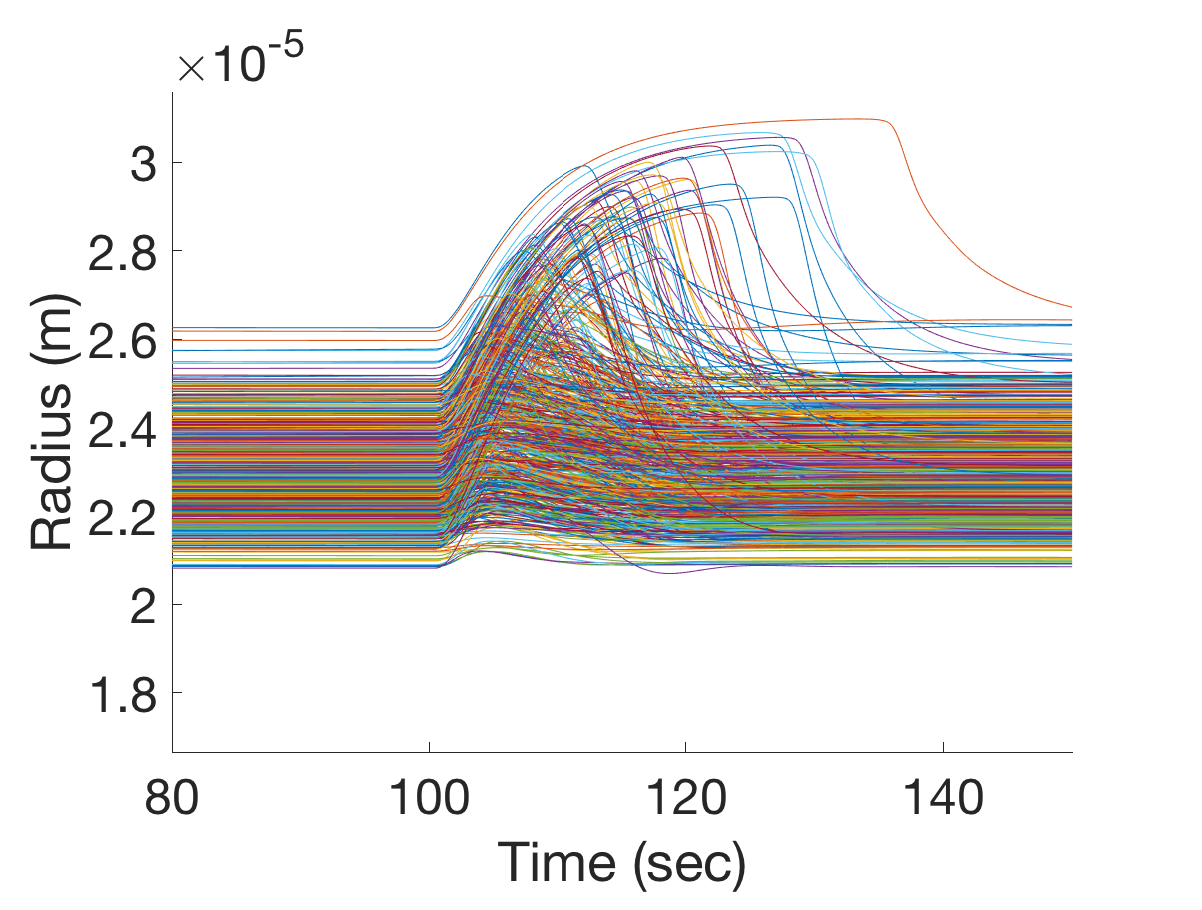
\includegraphics[width=.3 \textwidth]{Figures/Increase_with_Stim_Curves.eps}
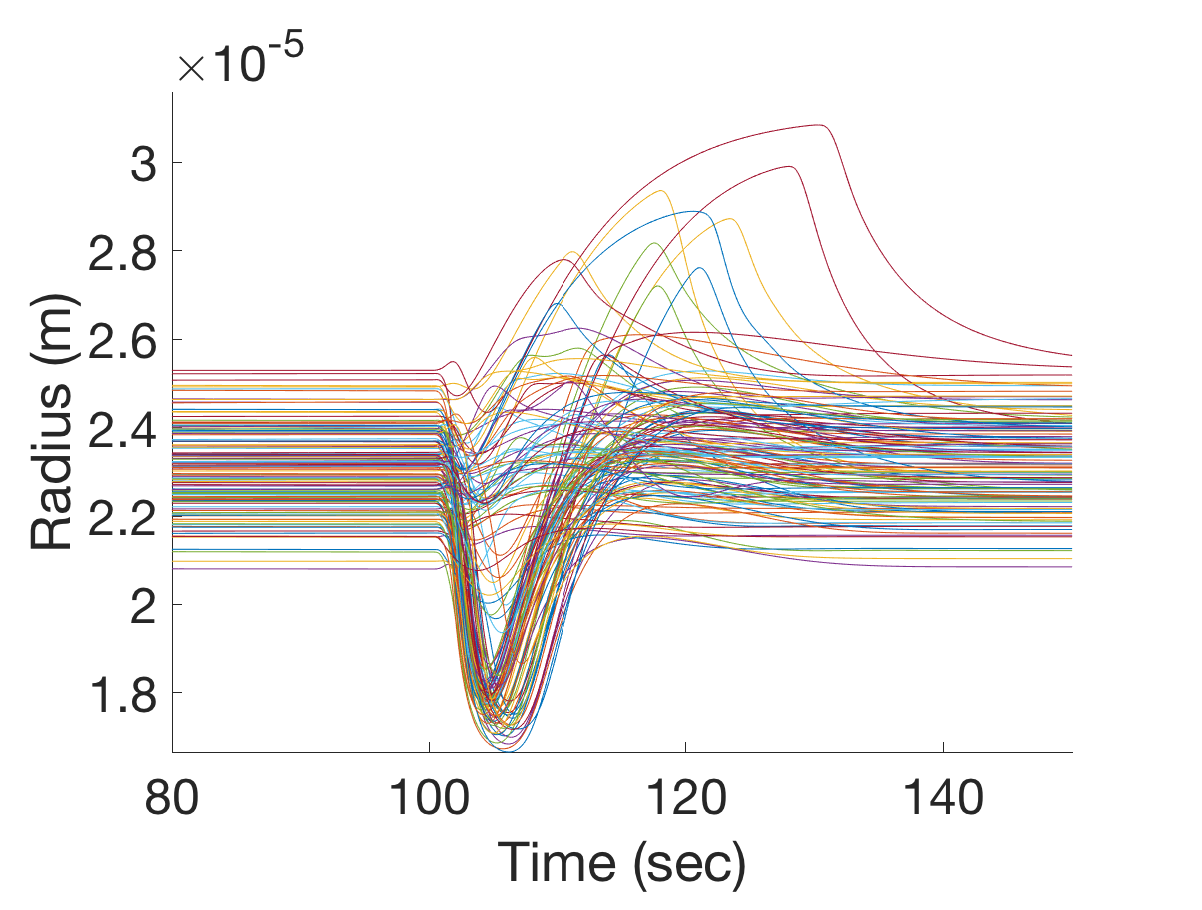
\includegraphics[width=.3 \textwidth]{Figures/Decrease_with_Stim_Curves.eps}
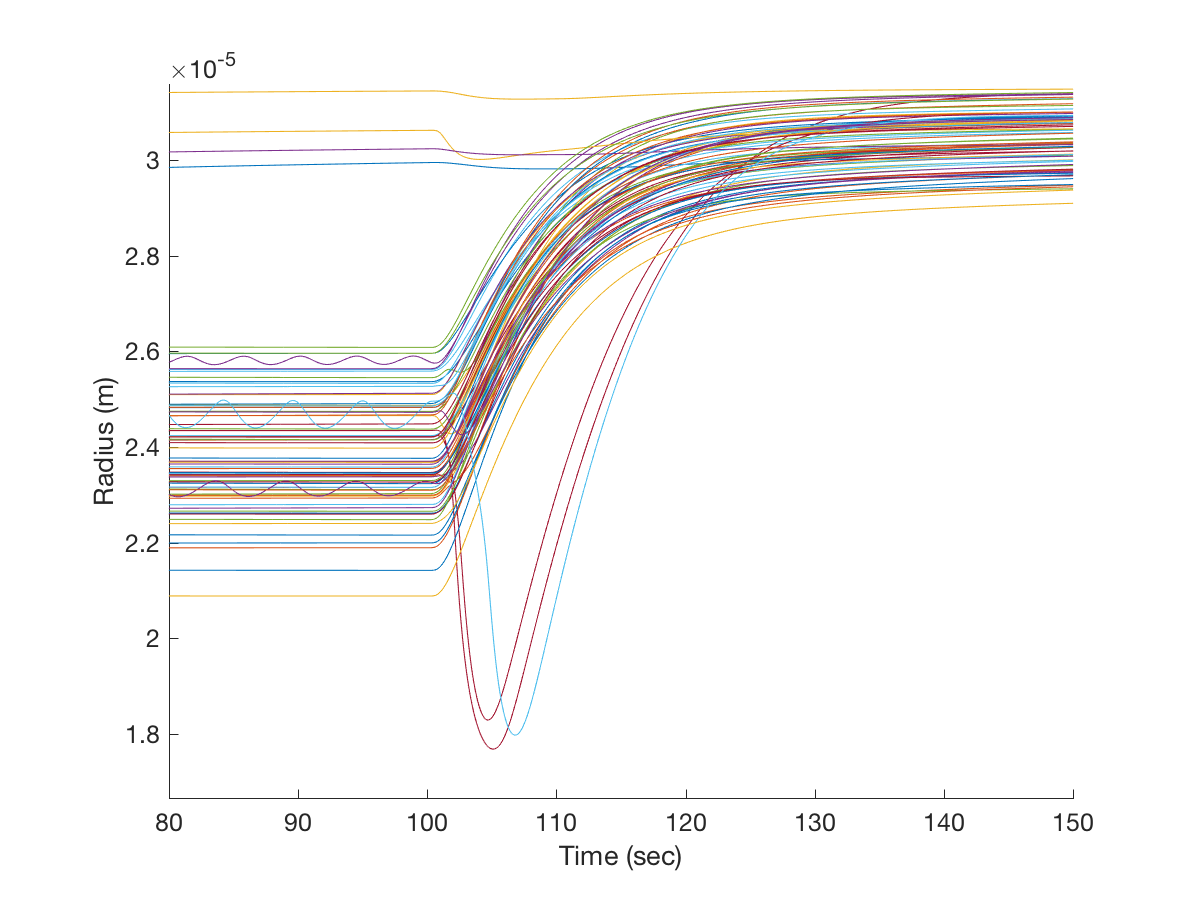
\includegraphics[width=.3 \textwidth]{Figures/Higher_Steady_State.eps}
\caption{Radii corresponding to samples (using the rectangular pulse stimulus). Left: curves an an increase in response to the stimulus; center: curves with a decrease in response to the stimulus; right: curves which settle in a different steady state.}
\label{solution_regimes}
\end{figure}

This article focuses on the non-pathological case, corresponding to the left panel of Figure~\ref{solution_regimes}, so we remove samples where the radius does not increase in response to the stimulus and decrease when it is removed. However, we recognise that a decrease in radius upon stimulation does not necessarily mean an incorrect result. Indeed these cases are of particular importance (due to the possibility of the existence of cortical spreading depression \cite{Kenny2018b}) and a topic of future research. This processing yields 660 samples for analysis when the rectangular pulse stimulus is applied and 438 samples when the experimental pulse stimulus is applied. The results presented below use these samples.

Exploration of the 660 retained samples indicate that ``pathological'' cases have higher probability when the parameter which shifts the activation variable for the \pot flux through the soma KDR channel is reduced;
 however, this parameter does not characterize the solution regime by itself; it is likely that the solution regime is characterized by a combination of several parameters. Further sampling and exploration is required to better understand the structure in parameter space which determine the solution regime.

The 160 parameters are indexed (purely for coding reasons) and are not to be taken as a ranked order. The tables of ranked parameters, given in the subsections below to summarize the most influential parameters, provide the parameters in the first column, their location in the Supplementary Material in the second column, and their total Sobol' indices for the experimental and rectangular pulses in the third and fourth columns, respectively. Each table contains the five most influential parameters for a given QoI, as measured by the total Sobol' indices for the experimental pulse. There are slight differences in the ordering of the less important parameters for the rectangular pulse and experimental pulse cases; the tables below report the ranking from the experimental pulse case. Both rectangular and experimental pulse cases agree on the ranking of the most influential parameters.

\subsection{Average ECS Potassium}
\label{sec:qoi_K_ECS_Mean}

Figure~\ref{fig:K_ECS_Mean_rect} and ~\ref{fig:K_ECS_Mean_exp} display results for the average of the ECS potassium, defined in equation (\ref{K_ECS_Mean}), for the rectangular pulse stimulus and experimental pulse stimulus, respectively. In the top left panels, predictions of the linear surrogate are plotted against the QoI values. The sensitivities $L_j$, $j=1,2,\dots,160$, are displayed in the top right panels. Predictions of the PC surrogate are plotted against the QoI values in the bottom left panels. The total Sobol' indices of the PC surrogate are given in the bottom right panels. Table~\ref{tab:K_ECS_Mean} reports the five most important parameters and their respective total Sobol' indices.

\begin{figure}[h]
\centering
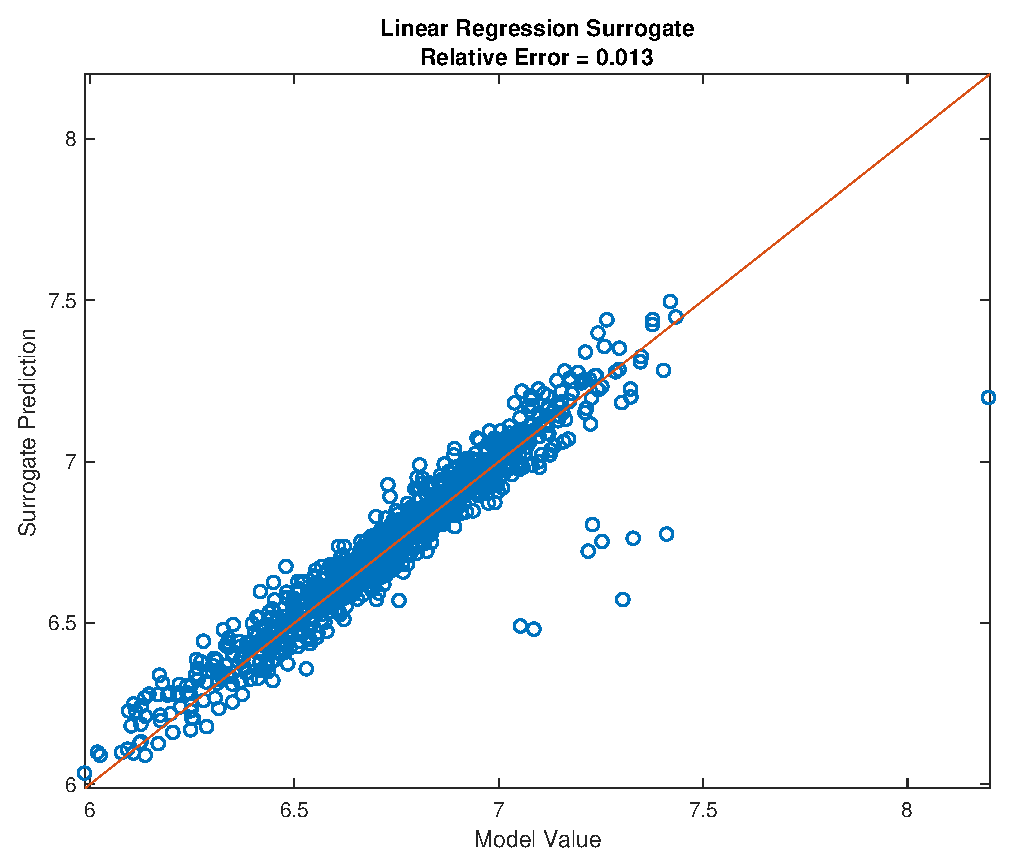
\includegraphics[width=.46 \textwidth]{Figures/K_ECS_Mean_QoI_LR_Prediction_Rectangular.eps}
\hspace{.1 cm}
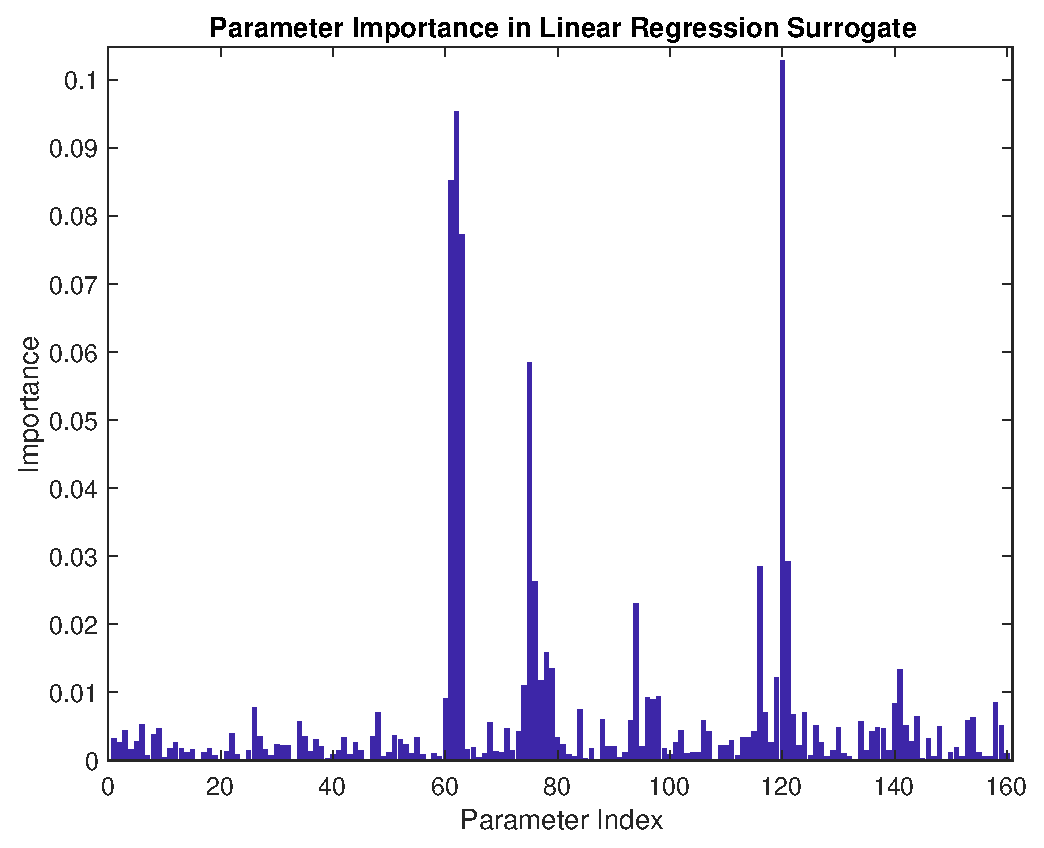
\includegraphics[width=.475 \textwidth]{Figures/K_ECS_Mean_QoI_LR_VI_Rectangular.eps} \\
\vspace{.2 cm}
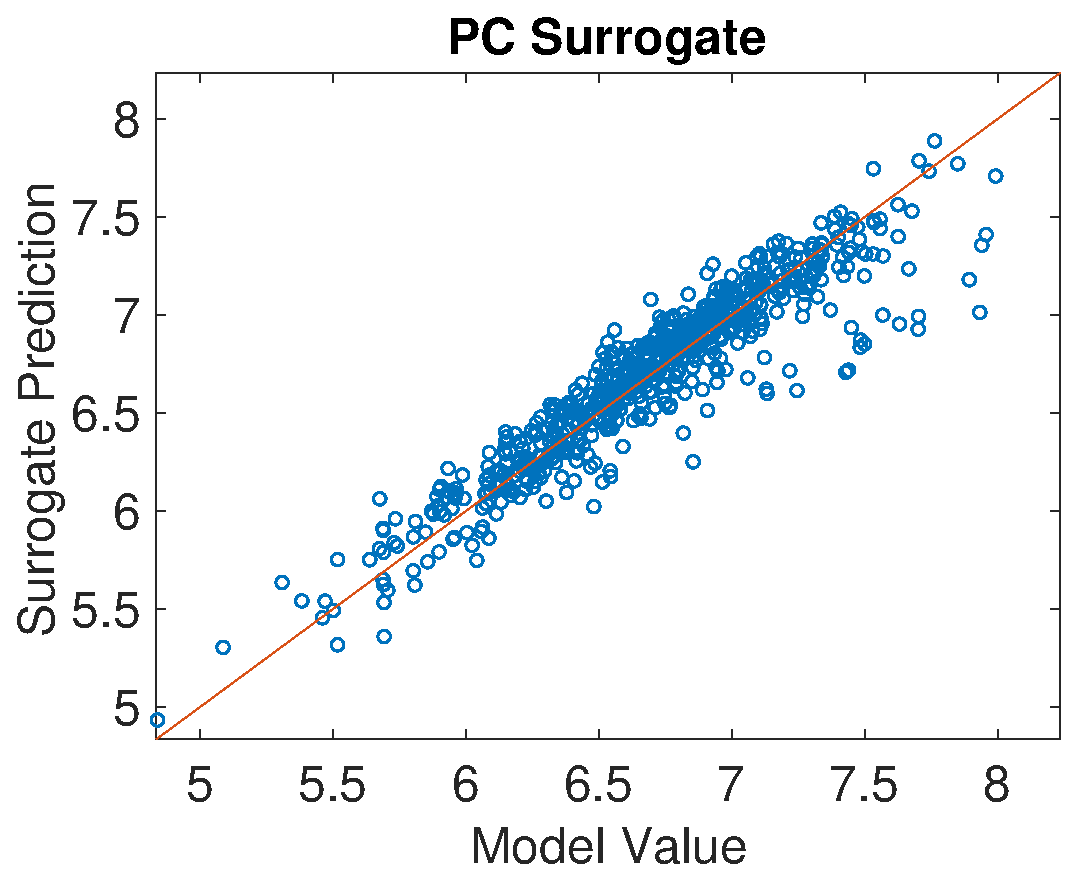
\includegraphics[width=.46 \textwidth]{Figures/K_ECS_Mean_QoI_PCE_Prediction_Rectangular.eps}
\hspace{.1 cm}
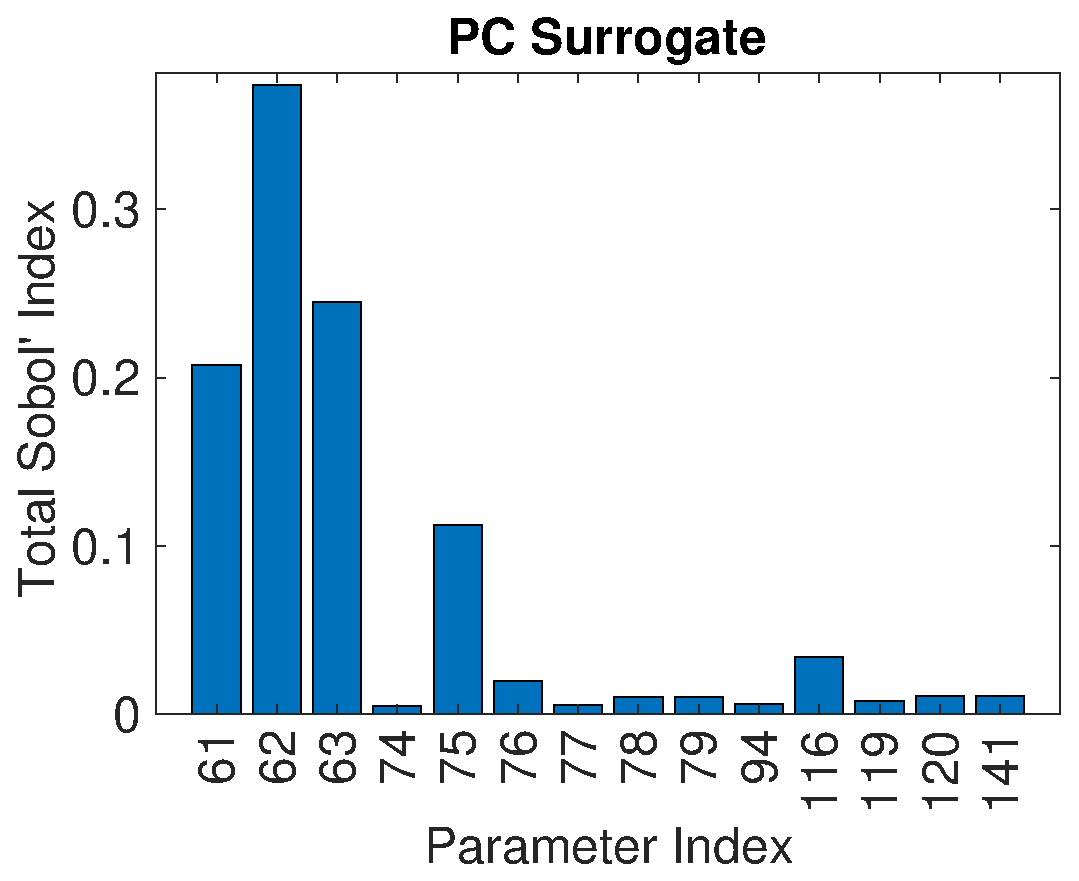
\includegraphics[width=.475 \textwidth]{Figures/K_ECS_Mean_QoI_PCE_SI_Rectangular.eps}
\caption{Average ECS potassium QoI with a rectangular pulse stimulus. From left to right and top to bottom: linear surrogate predictions, linear surrogate importance measure, PC surrogate predictions, total Sobol' indices for PC surrogate.}
\label{fig:K_ECS_Mean_rect}
\end{figure}
\begin{figure}[h]
\centering
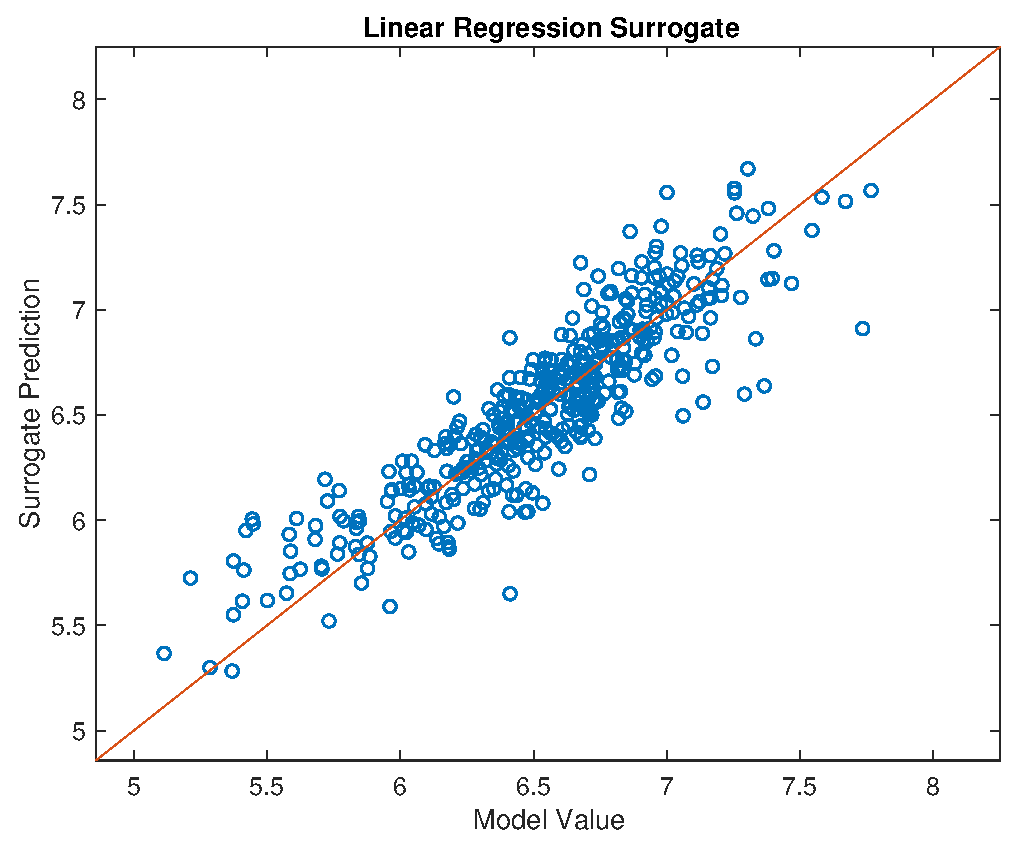
\includegraphics[width=.46 \textwidth]{Figures/K_ECS_Mean_QoI_LR_Prediction_Experimental.eps}
\hspace{.1 cm}
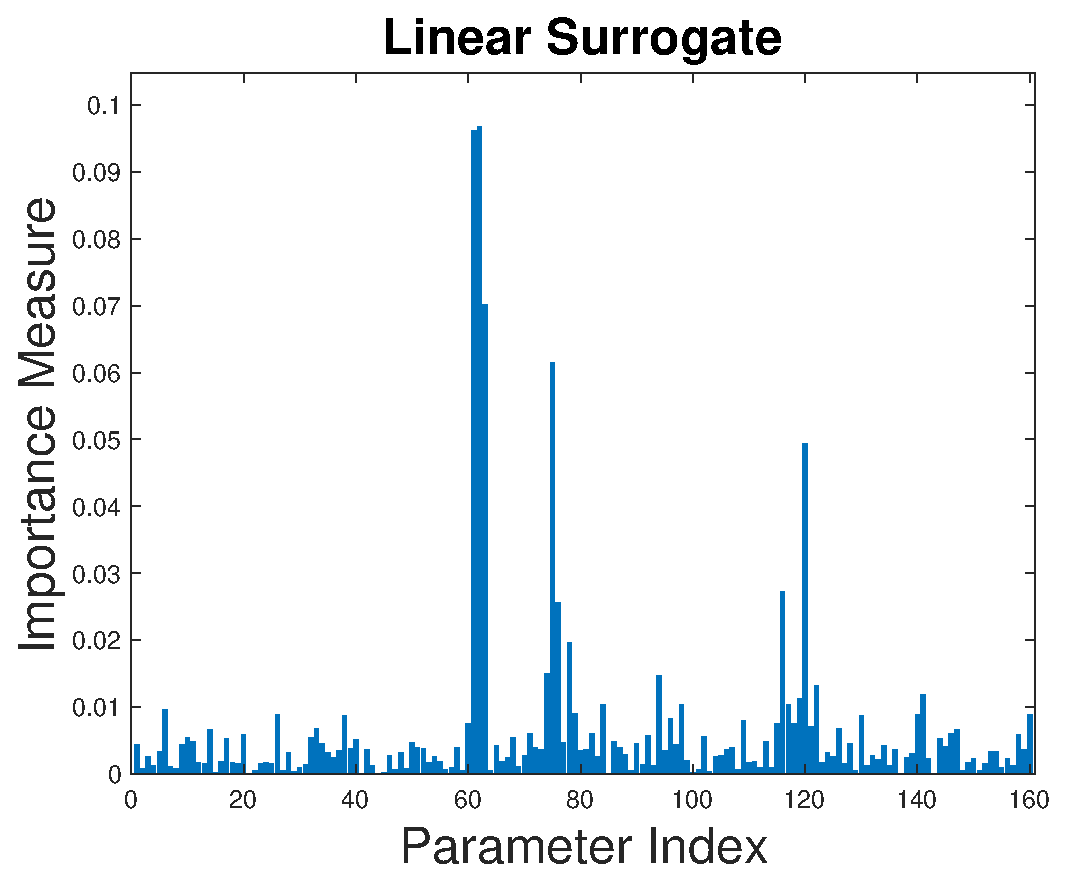
\includegraphics[width=.475 \textwidth]{Figures/K_ECS_Mean_QoI_LR_VI_Experimental.eps} \\
\vspace{.2 cm}
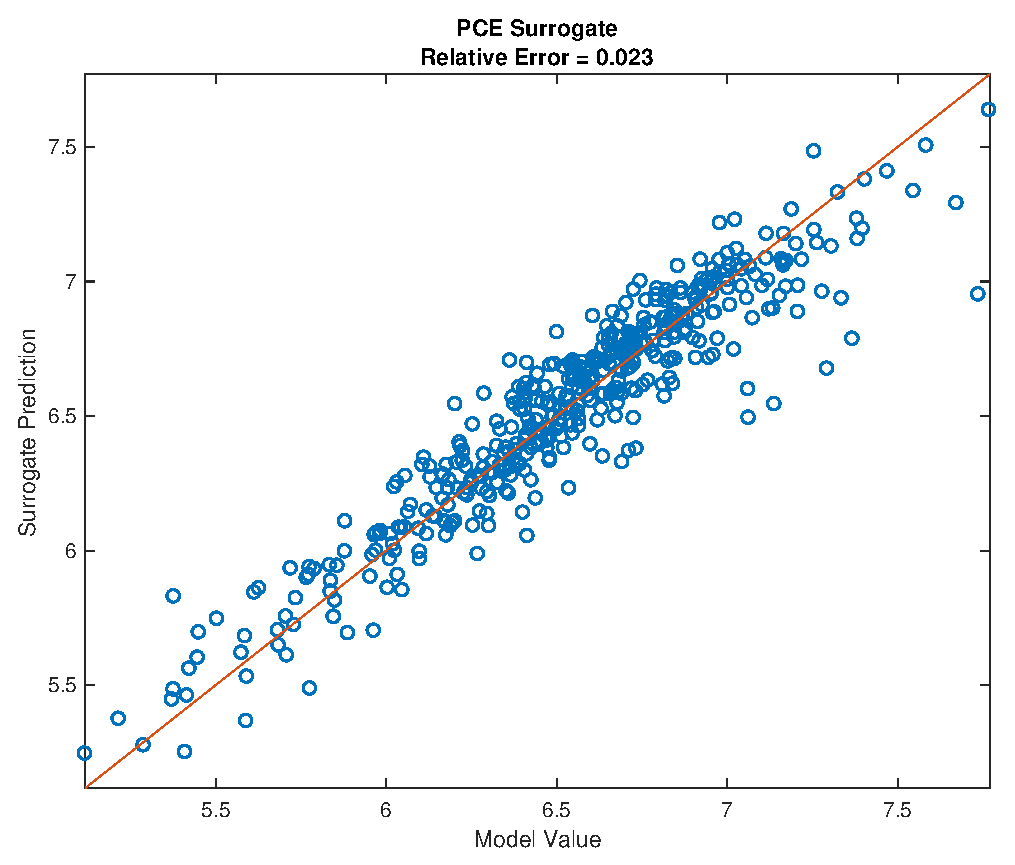
\includegraphics[width=.46 \textwidth]{Figures/K_ECS_Mean_QoI_PCE_Prediction_Experimental.eps}
\hspace{.1 cm}
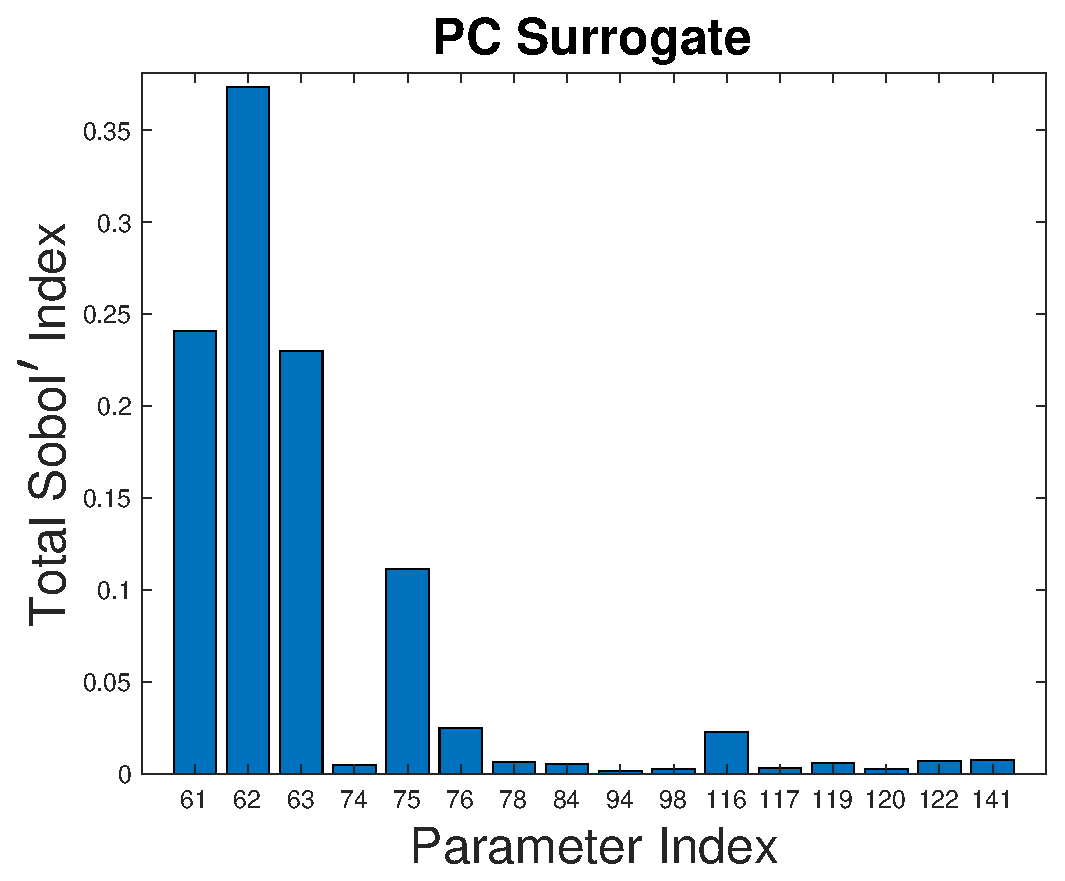
\includegraphics[width=.475 \textwidth]{Figures/K_ECS_Mean_QoI_PCE_SI_Experimental.eps}
\caption{Average ECS potassium QoI with experimental pulse stimulus. From left to right and top to bottom: linear surrogate predictions, linear surrogate importance measure, PC surrogate predictions, total Sobol' indices for PC surrogate.}
\label{fig:K_ECS_Mean_exp}
\end{figure}


%\begin{table}[h]
%\centering
%\ra{1.3}
%\begin{tabular}{cccc}
%\toprule
%Parameter Index & Identification & Total Sobol' Index (rect.) & Total Sobol' Index (exp.)\\
%\midrule
%62 & 0.143 in $m_{4\alpha}$ and $m_{4 \beta}$ &  0.3738 & 0.3732\\
%63 & 5.67 in $m_{4\alpha}$ and $m_{4 \beta}$  &  0.2449 & 0.2297\\
%61 & gKleak\_d in Neuron &0.2074 & 0.2409\\
%75 & 34.9 in $m_{6 \alpha}$ & 0.1124 & 0.1112\\
%116 & dhod in Neuron & 0.0342 & 0.0226\\
% \arrayrulecolor{black}\bottomrule
%\end{tabular}
%\caption{Most influential parameters for the ECS potassium QoI.}
%\label{tab:K_ECS_Mean}
%\end{table}
%\begin{table}[h]
%\centering
%\ra{1.3}
%\begin{tabular}{cccc}
%\toprule
%Parameter & Identification & Total Sobol' Index (exp.) & Total Sobol' Index (rect.)\\
%\midrule
%$\theta_{62}$ & scaling for activation variable in dendritic NaP channel  &  0.3732 & 0.3738\\
%$\theta_{61}$ & $K^+$ leak in  Neuron & 0.2409 & 0.2074\\
%$\theta_{63}$ &  shift in activation variable in dendritic NaP channel &  0.2297 & 0.2449 \\
%$\theta_{75}$ & scaling in dendritic KDR channel & 0.1112 & 0.1124\\
%$\theta_{76}$ & put identification & 0.0247 & 0.0198\\
% \arrayrulecolor{black}\bottomrule
%\end{tabular}
%\caption{Five most influential parameters for the ECS potassium QoI when the experimental pulse stimulus is applied. The leftmost column is the parameter, the left-center column identifies the parameter in the Supplementary Material, the right-center column is the total Sobol' index computed for the parameter using the experimental pulse stimulus, and the right column is the total Sobol' index computed for the parameter using the rectangular pulse stimulus.}
%\label{tab:K_ECS_Mean}
%\end{table}
\begin{table}[h]
\centering
\ra{1.3}
\begin{tabular}{cccc}
\toprule
Parameter & Identification in Supplementary Material & Total Sobol' Index (exp.) & Total Sobol' Index (rect.)\\
\midrule
$\theta_{62}$ & Nominal value 0.143 in equation (61) &  0.3732 & 0.3738\\
$\theta_{61}$ & $g_{K,leak_d}$ in equation (30) & 0.2409 & 0.2074\\
$\theta_{63}$ &  Nominal value 5.67 in equation (61) &  0.2297 & 0.2449 \\
$\theta_{75}$ & Nominal value 34.9 in equation (54) & 0.1112 & 0.1124\\
$\theta_{76}$ & Nominal value 0.2 in equation (54) & 0.0247 & 0.0198\\
 \arrayrulecolor{black}\bottomrule
\end{tabular}
\caption{Five most influential parameters for the average ECS potassium QoI when the experimental pulse stimulus is applied. The leftmost column is the parameter, the left-center column identifies the parameter in the Supplementary Material, the right-center column is the total Sobol' index computed for the parameter using the experimental pulse stimulus, and the right column is the total Sobol' index computed for the parameter using the rectangular pulse stimulus.}
\label{tab:K_ECS_Mean}
\end{table}
The first and third parameters in Table \ref{tab:K_ECS_Mean} are scaling and shift parameters ($\theta_{62}$ and $\theta_{63}$) for the activation gating variable, $m_4$ in the dendrite NaP channel respectively, whose ODE is defined as 
\begin{eqnarray}\label{eqn:m4}
\frac{dm_4}{dt}=m_{4 \alpha}(1-m_4)-m_{4 \beta}m_4, \nonumber \\
m_{4 \alpha}=  \frac{1}{6(1 + exp(-(\theta_{62}  v_d + \theta_{63})))},\nonumber \\
m_{4 \beta}= \frac{exp(-(\theta_{62} v_d + \theta_{63}))}{6(1 + exp(-(\theta_{62} v_d + \theta_{63})))}.
\end{eqnarray}
where $v_d$ is the dendrite membrane potential. \\
The nominal values of $\theta_{62}$ and $\theta_{63}$ are 0.143 and 5.67, respectively. These effectively define the characteristic time scale and forcing function in the rate equation for the open  probability of the persistent sodium channel. The second most important parameter determines the strength of the  conductance in the \pot leak ion channel. The fourth and fifth parameters, $\theta_{75}$ and $\theta_{76}$, are the shift and scale of the neuron membrane potential in the ODE for the activation variable for the  K flux through dendritic KDR channel, defined as 
\begin{eqnarray}\label{eqn:m6}
m_{6  \alpha}     = \theta_{74} \left(\frac{v_d + \theta_{75}}{1 - exp(-(\theta_{76}  v_d + \theta_{76} \theta_{75}))} \right), 
\end{eqnarray}
where the nominal values for $\theta_{74}, \theta_{75}$, and $\theta_{76}$ are 0.016, 34.9, and 0.2, respectively. 

The results for this specific QoI are similar for both the rectangular pulse and experimental pulse stimulus. In both cases, the QoI is approximated with reasonable accuracy by a linear surrogate and with higher accuracy by the PC surrogate. The most important parameters are shared in both cases. Notice that parameter $\theta_{120}$, defined in \eqref{eqn:buff}, appears to be important in the linear surrogate but unimportant in the PC surrogate. This is because it is strongly correlated with parameter $\theta_{121}$ (also defined in defined in \eqref{eqn:buff}), see Figure~\ref{steady_states}, and as a result the coefficient in the linear surrogate may be very large because its effect is offset by the effect of $\theta_{121}$. To decorrelate inputs, the PC surrogate is build with only $\theta_{120}$ instead of both $\theta_{120}$ and $\theta_{121}$. It subsequently has minimal importance.

We also analysed another QoI for the ECS potassium, namely, its maximum over the interval of stimulation. The results are not reported because of their similarity to the average ECS potassium QoI results given above.

The remaining two QoIs also present very similar results for both the rectangular pulse and experimental pulse stimulus. In the interest of conciseness, we only present figures corresponding to the experimental pulse stimulus for these two QoIs; Tables~\ref{tab:qoi_vol_flow} and ~\ref{tab:qoi_AM_AMp_Min} give results for both stimuli. 

\subsection{Average Volumetric Flow Rate}
Figure~\ref{fig:qoi_vol_flow_exp} displays results for the average volumetric flow rate in the cerebral tissue defined by (\ref{vol_flow}) in the same manner as Figures~\ref{fig:K_ECS_Mean_rect} and \ref{fig:K_ECS_Mean_exp}.   Table~\ref{tab:qoi_vol_flow} reports the five most important parameters and their total Sobol' indices. Unsurprisingly, the parameter list contains values found in the SMC/EC compartment of the full model. However, the topmost parameter, $\theta_{141}$, is associated with the conductance of the inwardly rectifying SMC KIR channel, $g_{KIR}$, defined as a function of both membrane potential $v_{SMC}$ and the \pot concentration in the perivascular space $[K^+]_{PVS}$, given by 
\begin{eqnarray}
g_{KIR}=exp\left( \theta_{142} v_{SMC}+\theta_{140}[K^+]_{PVS}-\theta_{141}\right)  \label{eqn:gkir}
\end{eqnarray}
as shown in \cite{Dormanns2015} fitting to the data of \cite{Filosa2006}. $\theta_{141}$ shifts the conductance to the right for constant $[K^+]_{PVS}$  concentration in the perivascular space. The second parameter in Table \ref{tab:qoi_vol_flow}, $\theta_{158}$ (found in the wallmechanics section of the model) determines the strength of influence of cytosolic $[Ca^{2+}]$ in determining the reaction rate of phosphorylation of myosin \cite{Hai1988}. Although not especially important, the third listed parameter $\theta_{139}$ shifts the Nernst potential for the KIR channel to the right in the equation
\begin{eqnarray}
v_{KIR}=\theta_{138} [K^+]_{PVS}-\theta_{139}. \label{vkir}
\end{eqnarray}

\begin{figure}[h!]
\centering
%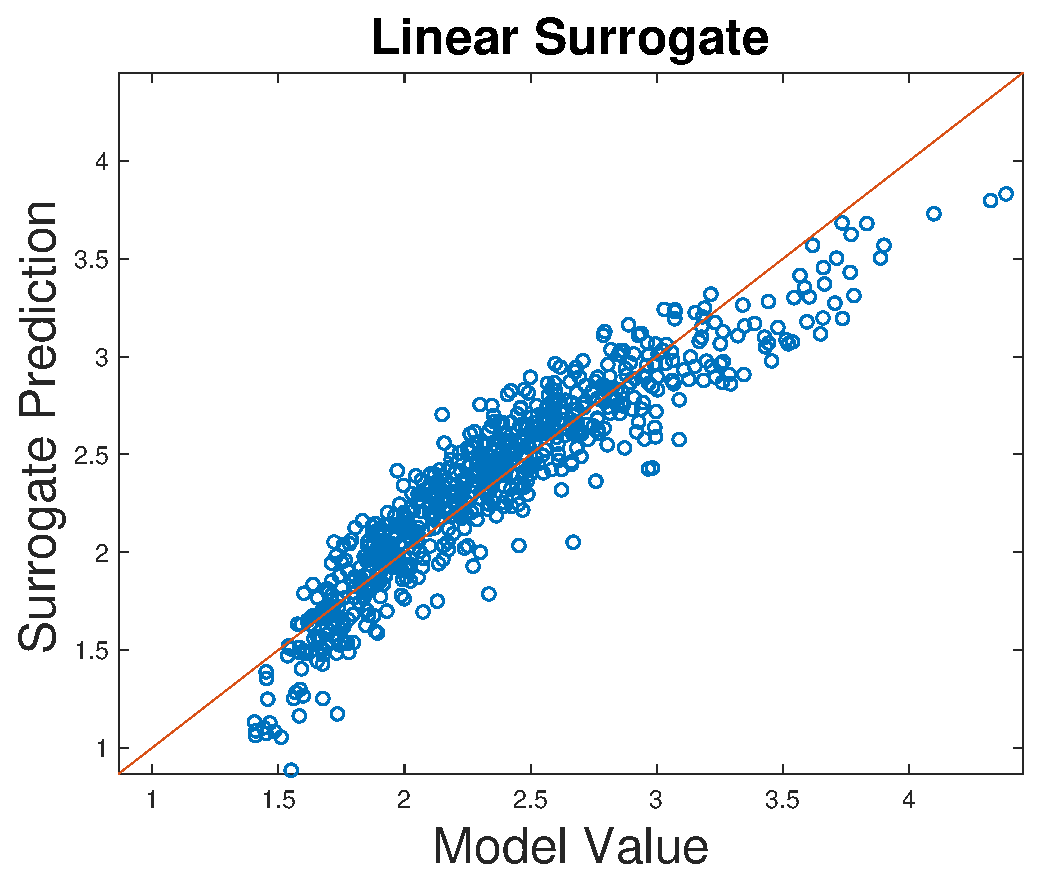
\includegraphics[width=.24 \textwidth]{Figures/Vol_Flow_QoI_LR_Prediction_Rectangular.eps}
%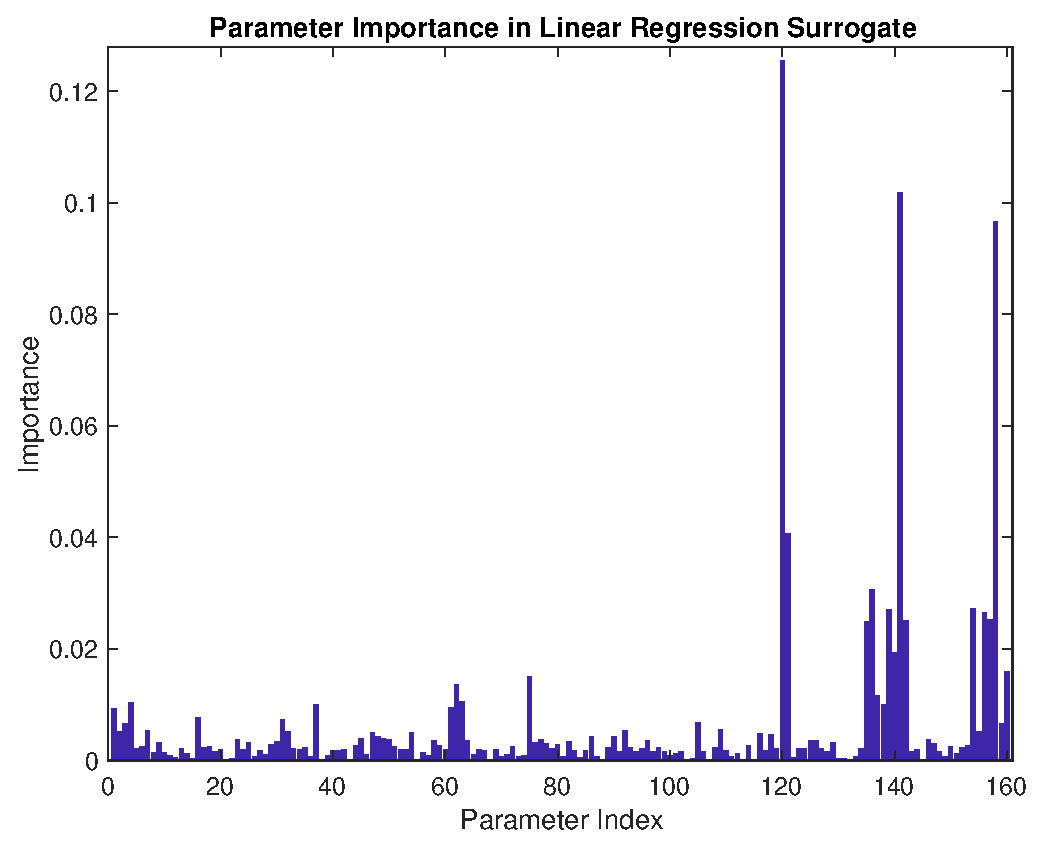
\includegraphics[width=.24 \textwidth]{Figures/Vol_Flow_QoI_LR_VI_Rectangular.eps}
%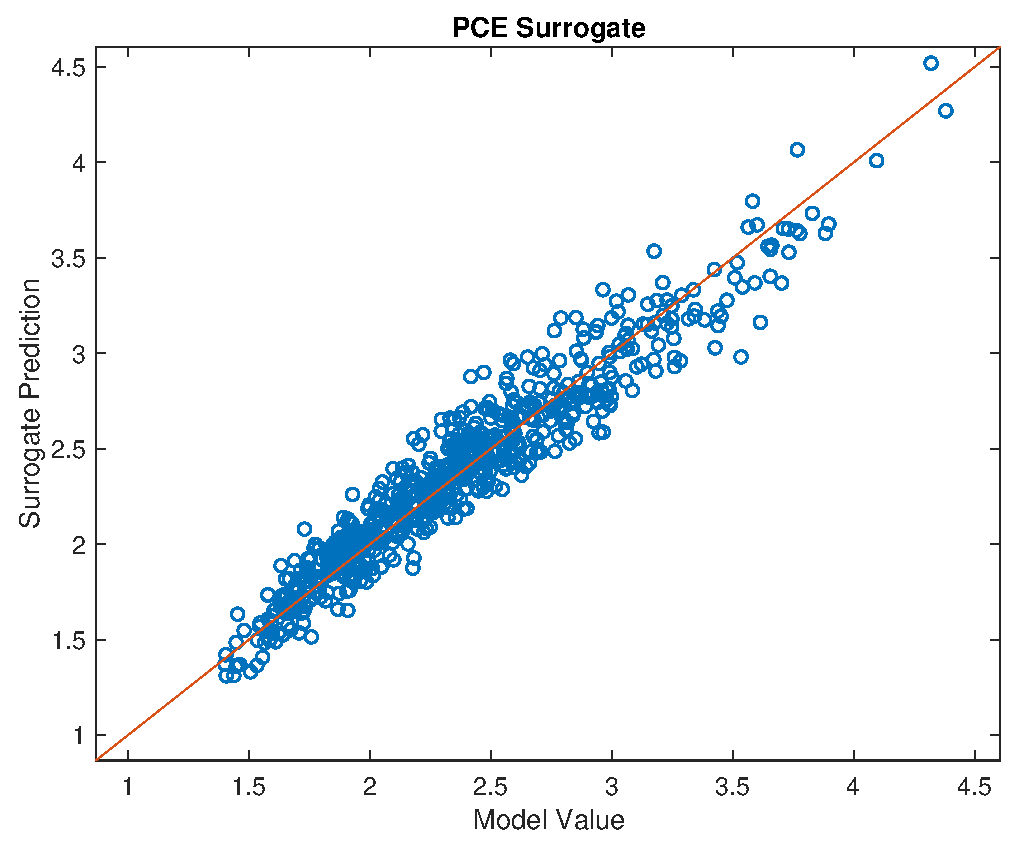
\includegraphics[width=.24 \textwidth]{Figures/Vol_Flow_QoI_PCE_Prediction_Rectangular.eps}
%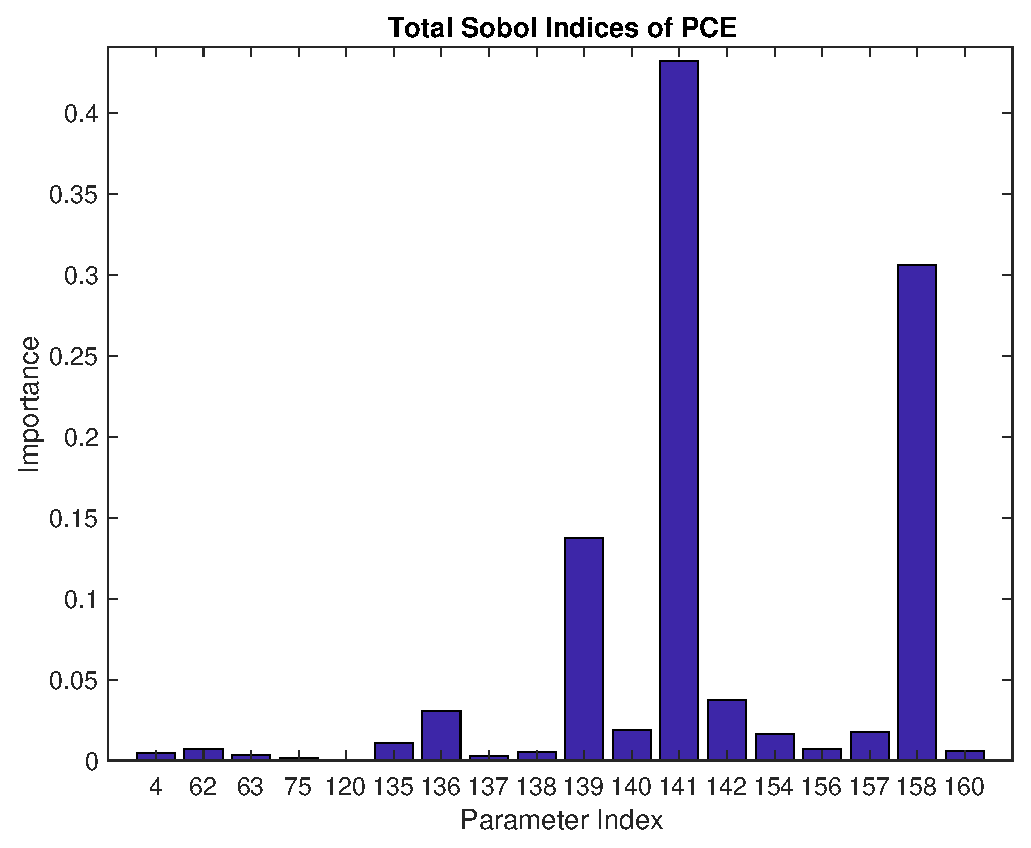
\includegraphics[width=.24 \textwidth]{Figures/Vol_Flow_QoI_PCE_SI_Rectangular.eps}\\
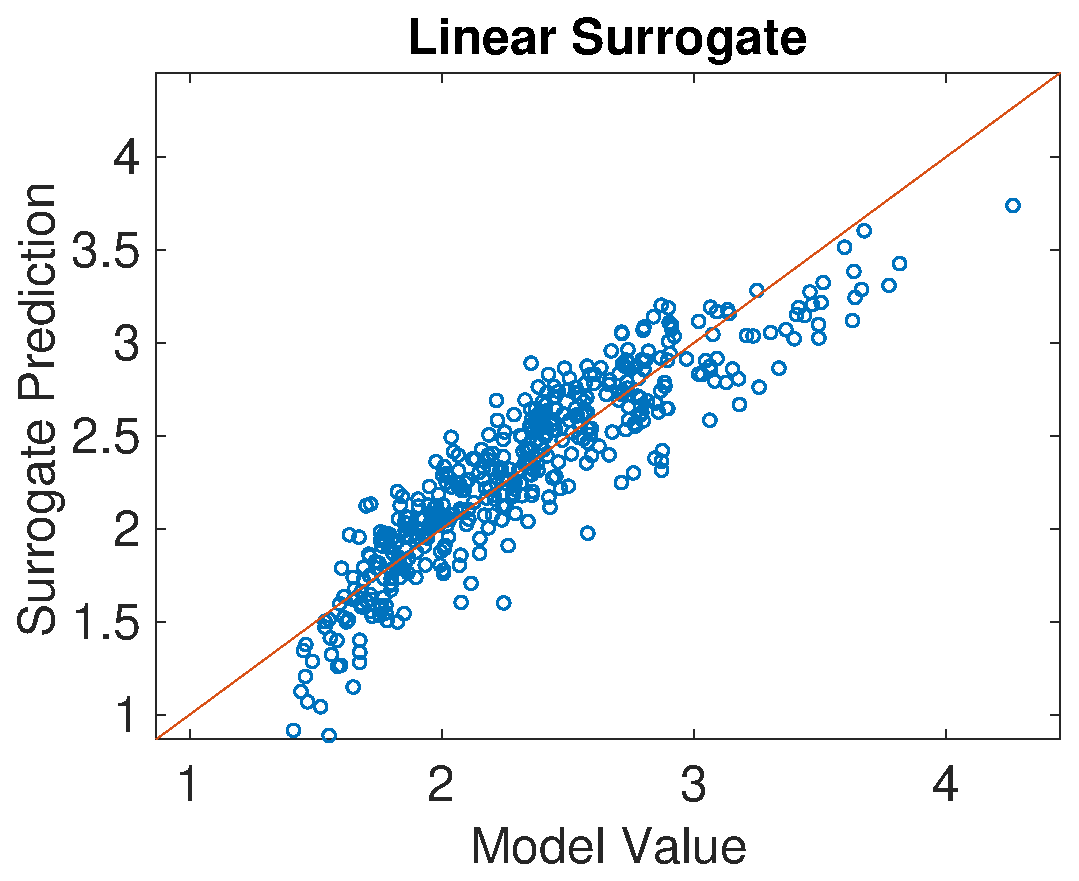
\includegraphics[width=.46 \textwidth]{Figures/Vol_Flow_QoI_LR_Prediction_Experimental.eps}
\hspace{.1 cm}
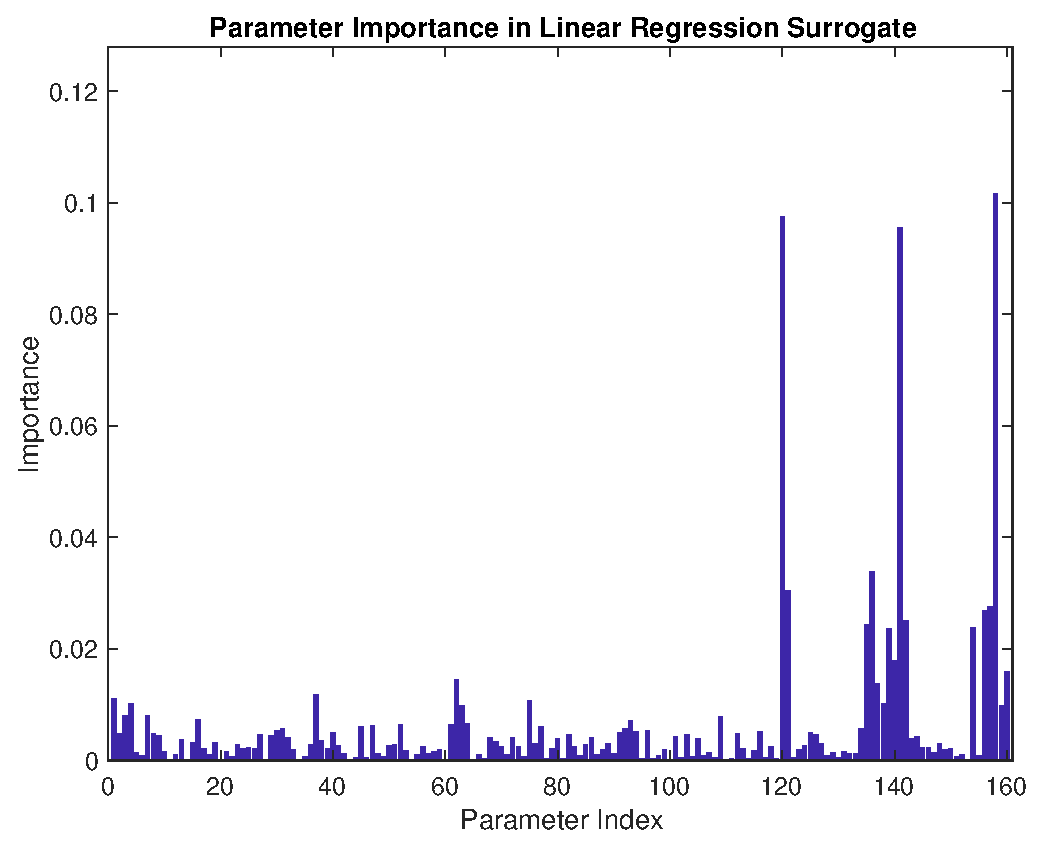
\includegraphics[width=.475 \textwidth]{Figures/Vol_Flow_QoI_LR_VI_Experimental.eps} \\
\vspace{.2 cm}
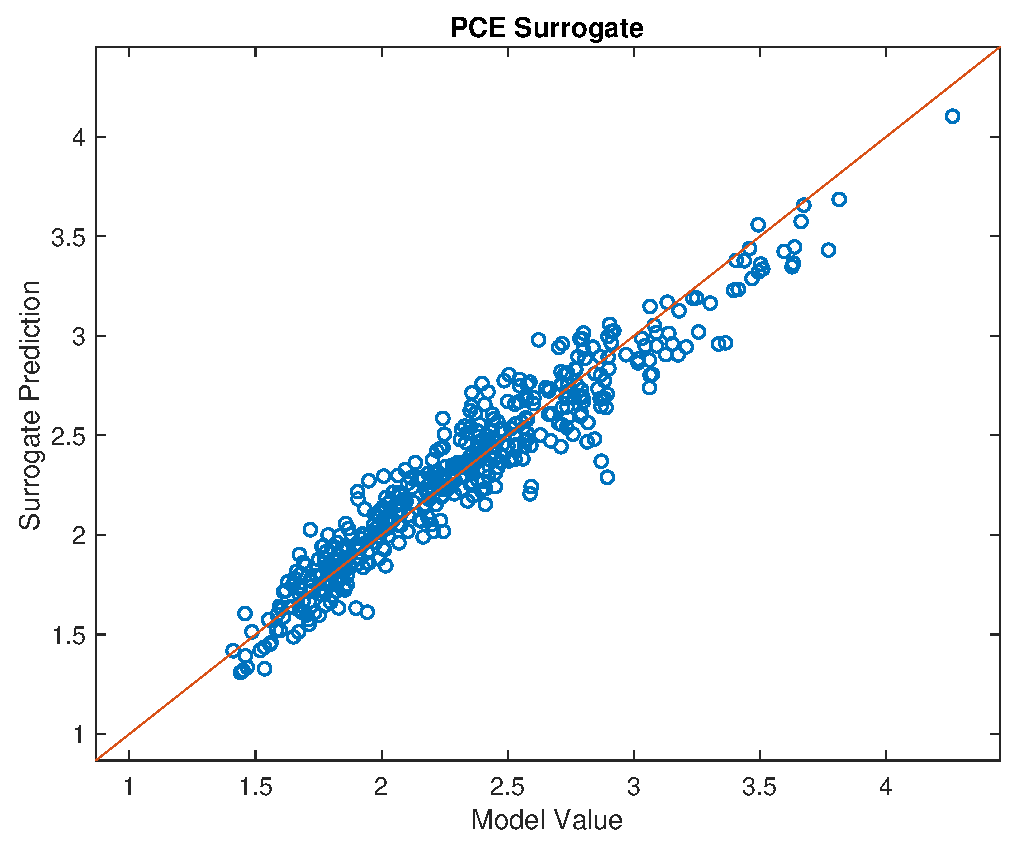
\includegraphics[width=.46 \textwidth]{Figures/Vol_Flow_QoI_PCE_Prediction_Experimental.eps}
\hspace{.1 cm}
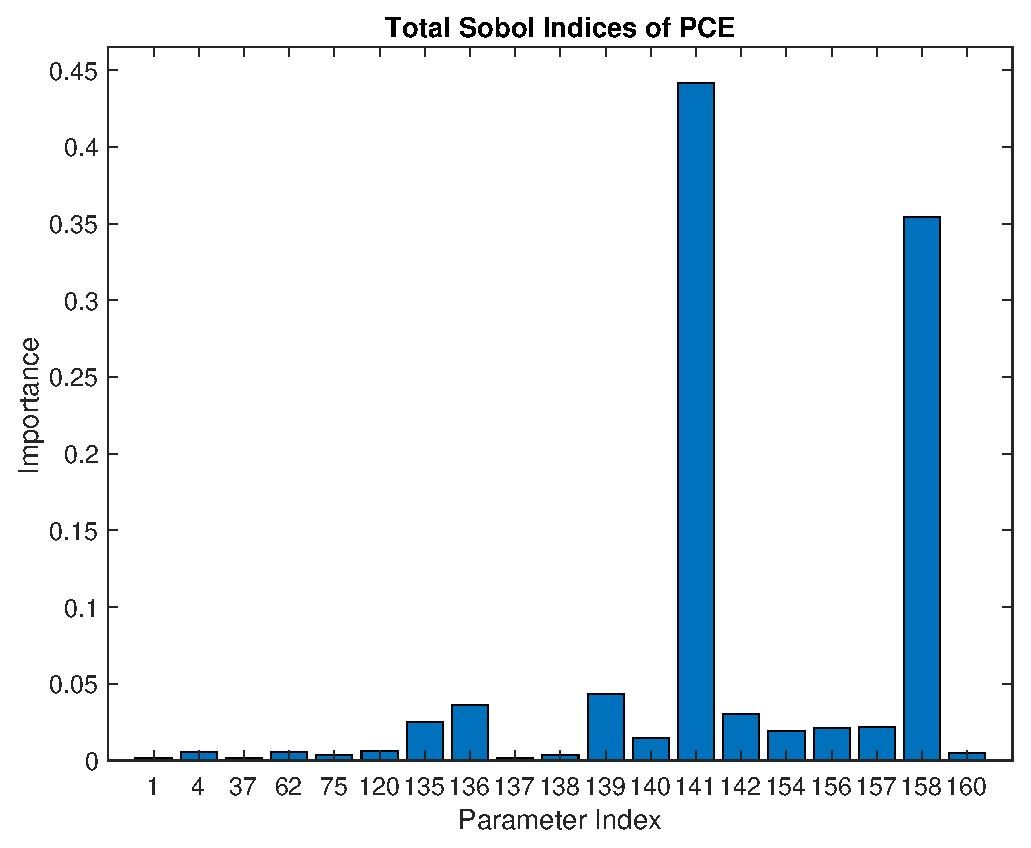
\includegraphics[width=.475 \textwidth]{Figures/Vol_Flow_QoI_PCE_SI_Experimental.eps}
\caption{Average volumetric flow rate QoI with experimental pulse stimulus. From left to right and top to bottom: linear surrogate predictions, linear surrogate importance measure, PC surrogate predictions, total Sobol' indices for PC surrogate.}
\label{fig:qoi_vol_flow_exp}
\end{figure}

We again observe reasonably accurate fits by a linear surrogate and improved accuracy by a PC surrogate. The surrogate predictions and important parameters for the rectangular pulse and experimental pulse closely agree.  As in Subsection~\ref{sec:qoi_K_ECS_Mean}, parameter $\theta_{120}$ appears important in the linear surrogate but unimportant in the PC surrogate.

\begin{table}[h]
\centering
\ra{1.3}
\begin{tabular}{cccc}
\toprule
Parameter & Identification in Supplementary Material & Total Sobol' Index (exp.) & Total Sobol' Index (rect.) \\
\midrule
$\theta_{141}$ &  $z_4$ in equation (149)  & 0.4420 & 0.4561\\
$\theta_{158}$ & $n_{cross}$ in equation (214)   & 0.3544 & 0.3311\\ 
 $\theta_{139}$ & $z_2$ in equation (148)  & 0.0436 & 0.0529\\
$\theta_{136}$ & $G_{K_i}$ in equation (149)   & 0.0362 & 0.0305\\
$\theta_{142}$ & $z_5$ in equation (149)   &  0.0305 & 0.0351\\
   \arrayrulecolor{black}\bottomrule
\end{tabular}
\caption{Five most influential parameters for the average volumetric flow rate QoI when the experimental pulse stimulus is applied. The leftmost column is the parameter, the left-center column identifies the parameter in the Supplementary Material, the right-center column is the total Sobol' index computed for the parameter using the experimental pulse stimulus, and the right column is the total Sobol' index computed for the parameter using the rectangular pulse stimulus.}
\label{tab:qoi_vol_flow}
\end{table}

\subsection{$[AM+AM_p]_{min}$}

Figure~\ref{fig:qoi_AM_AMp_Min_exp} displays results for the minimum of the combined concentration of the actin myosin complex with the experimental pulse stimulus. Table~\ref{tab:qoi_AM_AMp_Min} reports the five most important parameters and their total Sobol' indices. By comparing Table~\ref{tab:qoi_AM_AMp_Min} and Table~\ref{tab:qoi_vol_flow}, we see that the $[AM+AM_p]_{min}$ and average volumetric flow rate QoIs share four of their five most important parameters. Although at first analysis this should not be surprising it does suggest that the reaction rates of the actin myosin model for vessel contraction/dilation are relatively insensitive to finding the minimum of the contraction force and that the KIR ion channel is a vital component of the model. 
\begin{figure}[h]
\centering
%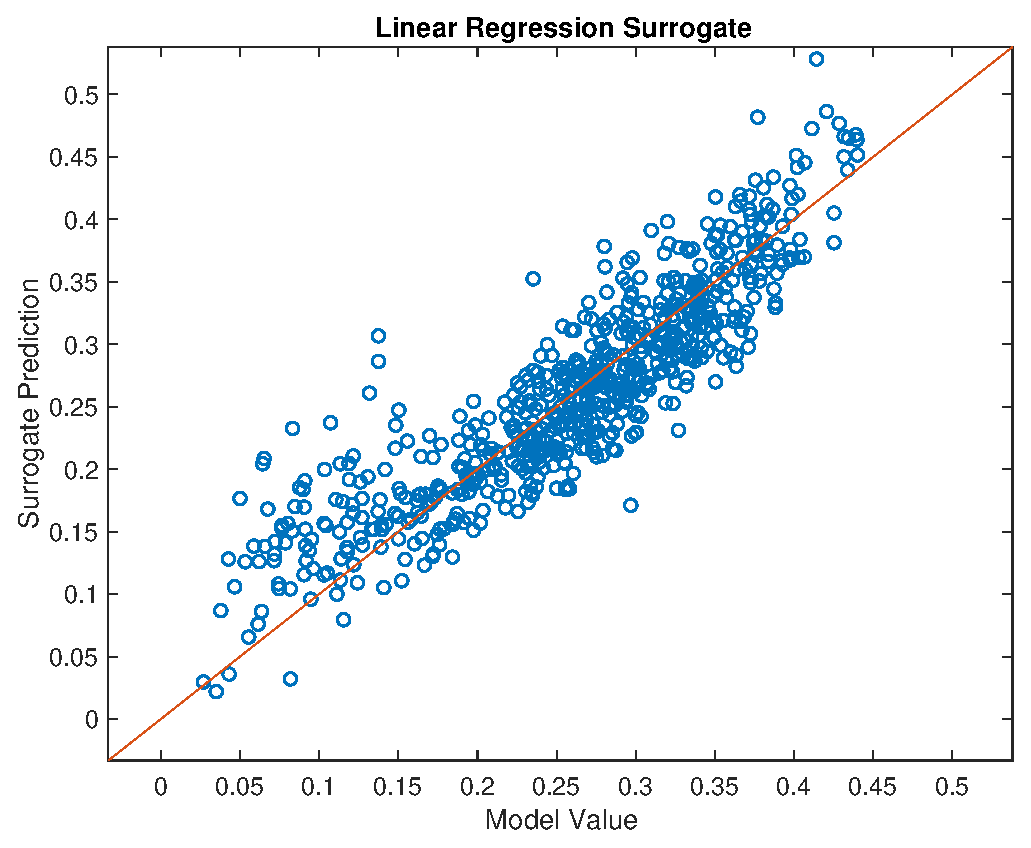
\includegraphics[width=.24 \textwidth]{Figures/AM_AMp_Min_QoI_LR_Prediction_Rectangular.eps}
%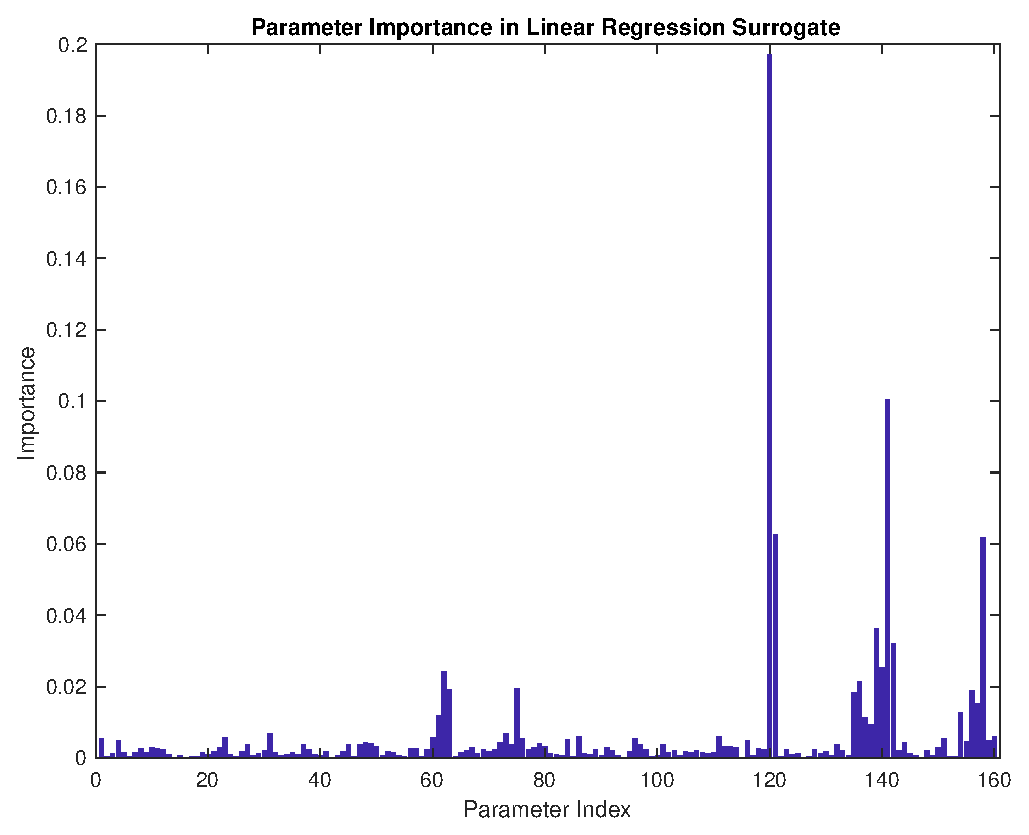
\includegraphics[width=.24 \textwidth]{Figures/AM_AMp_Min_QoI_LR_VI_Rectangular.eps}
%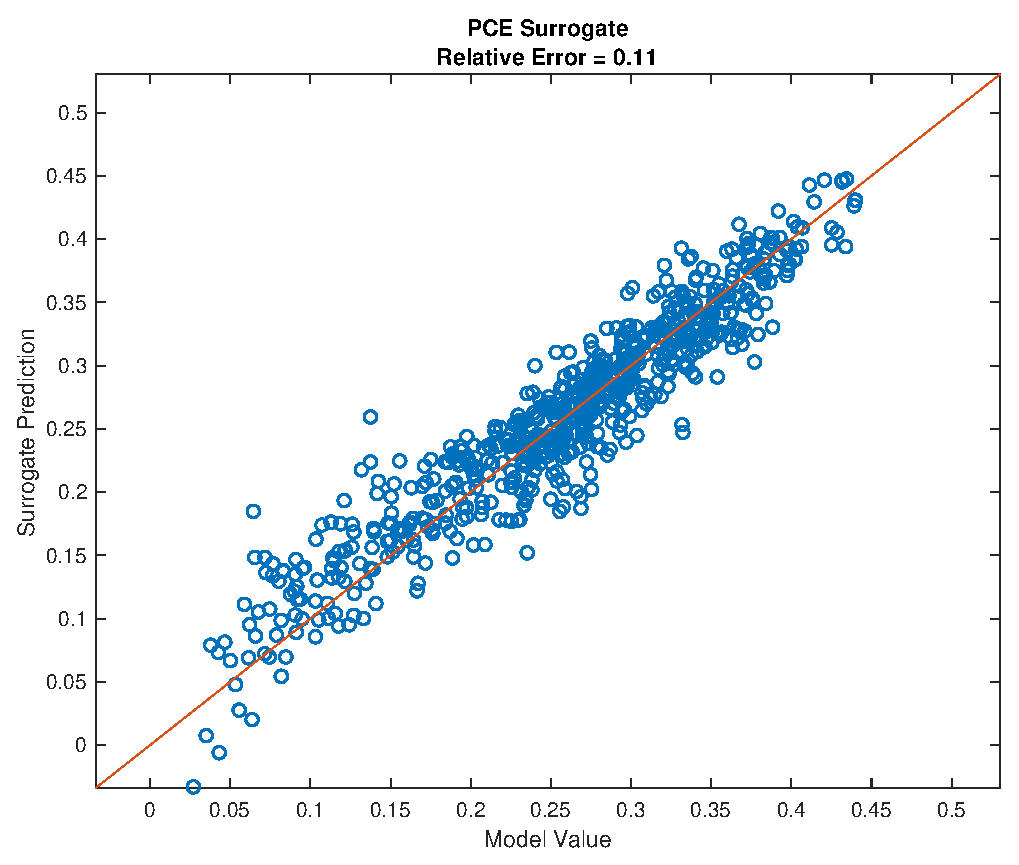
\includegraphics[width=.24 \textwidth]{Figures/AM_AMp_Min_QoI_PCE_Prediction_Rectangular.eps}
%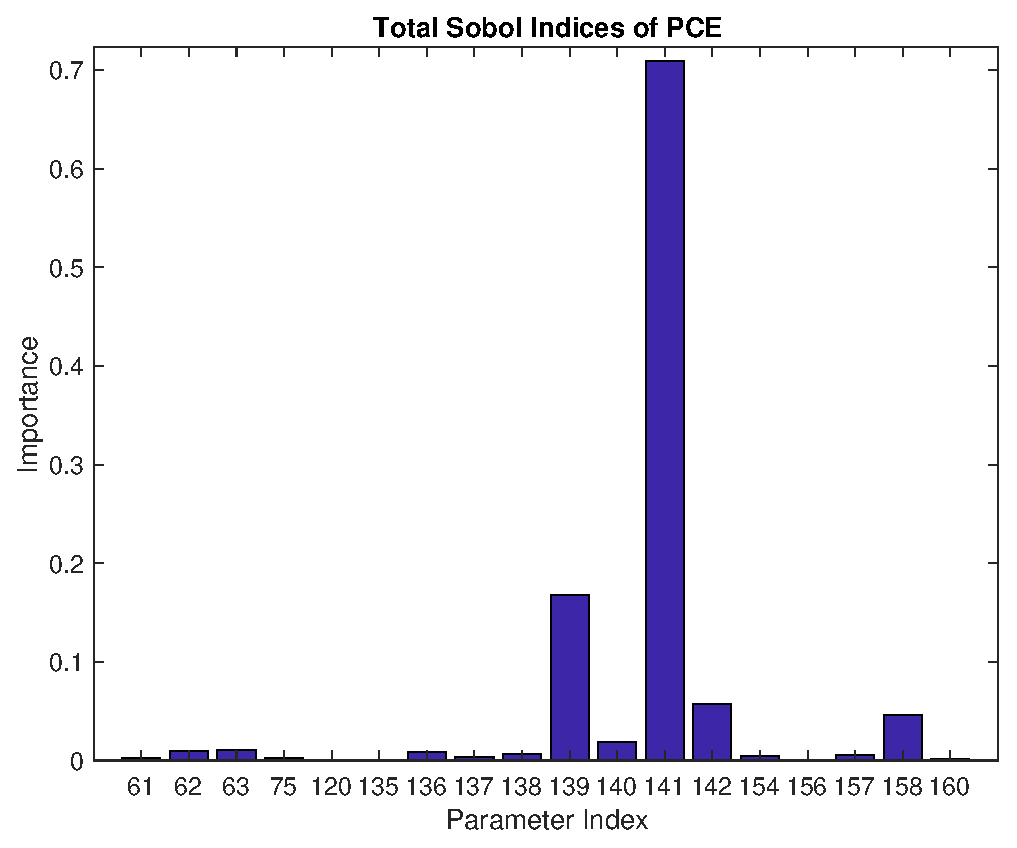
\includegraphics[width=.24 \textwidth]{Figures/AM_AMp_Min_QoI_PCE_SI_Rectangular.eps}\\
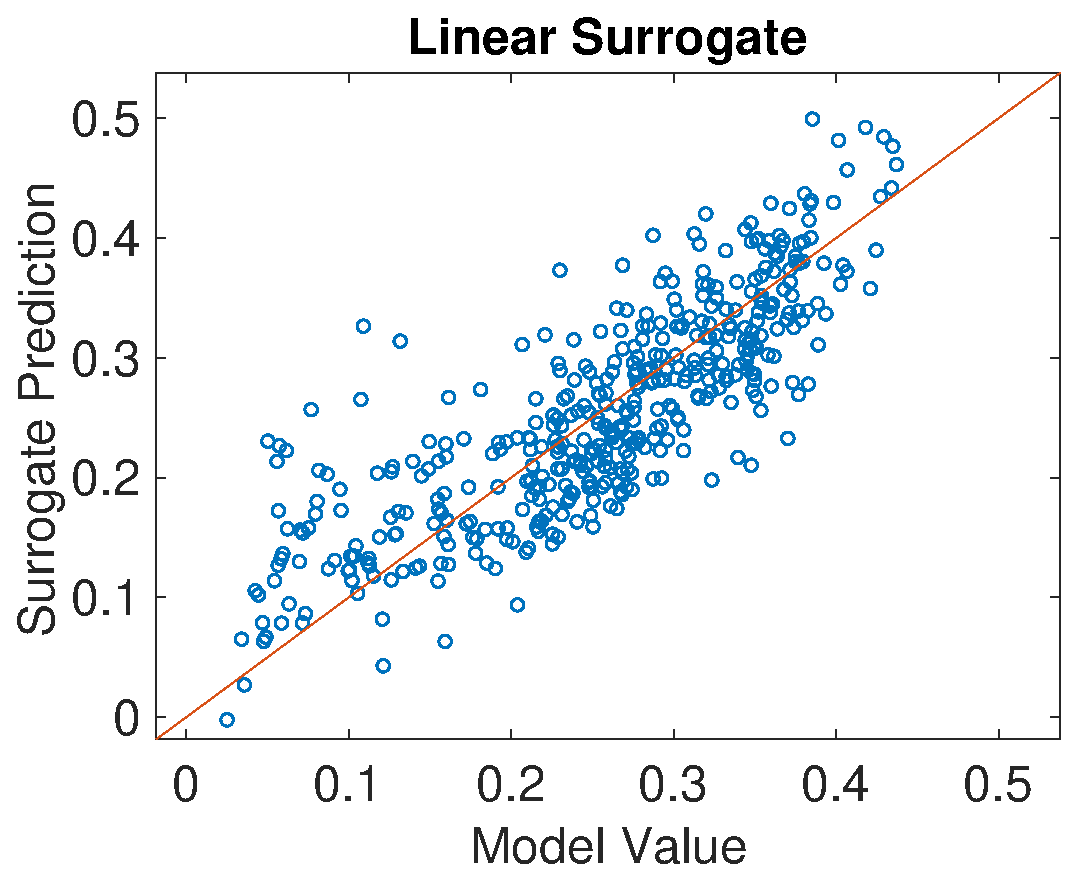
\includegraphics[width=.46 \textwidth]{Figures/AM_AMp_Min_QoI_LR_Prediction_Experimental.eps}
\hspace{.1 cm}
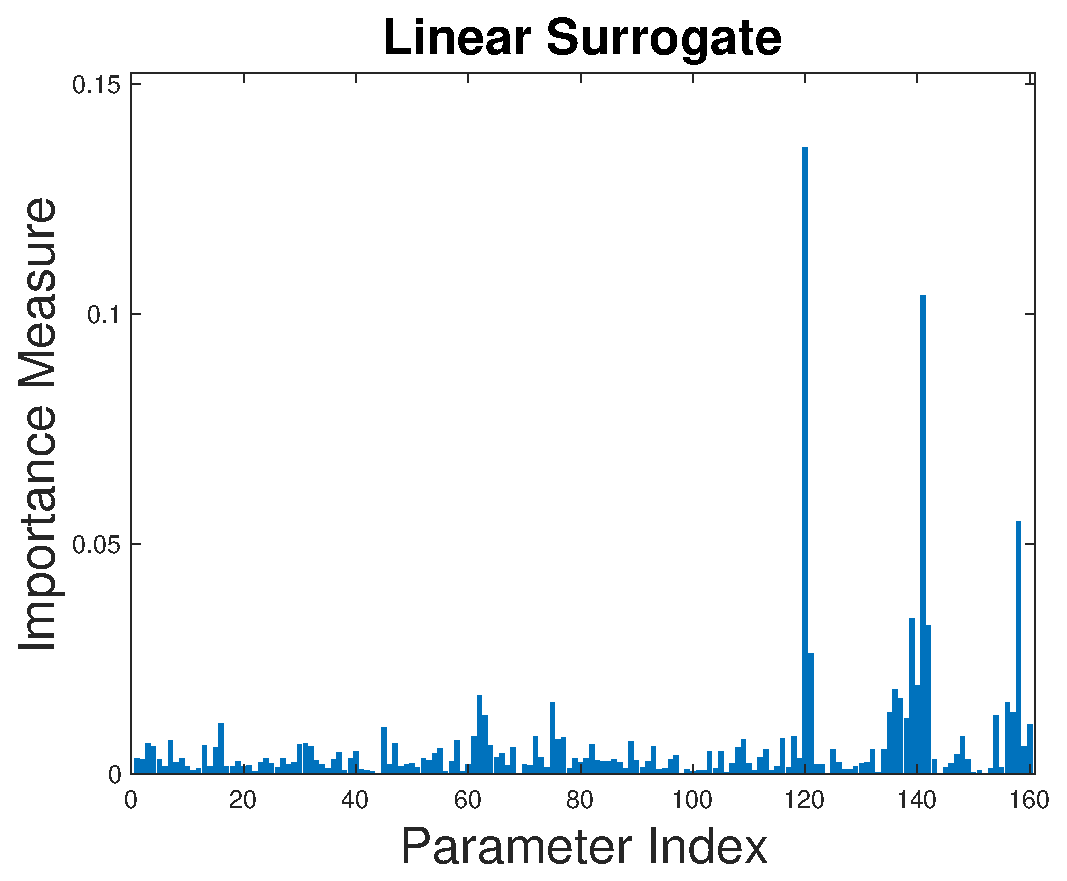
\includegraphics[width=.475 \textwidth]{Figures/AM_AMp_Min_QoI_LR_VI_Experimental.eps} \\
\vspace{.2 cm}
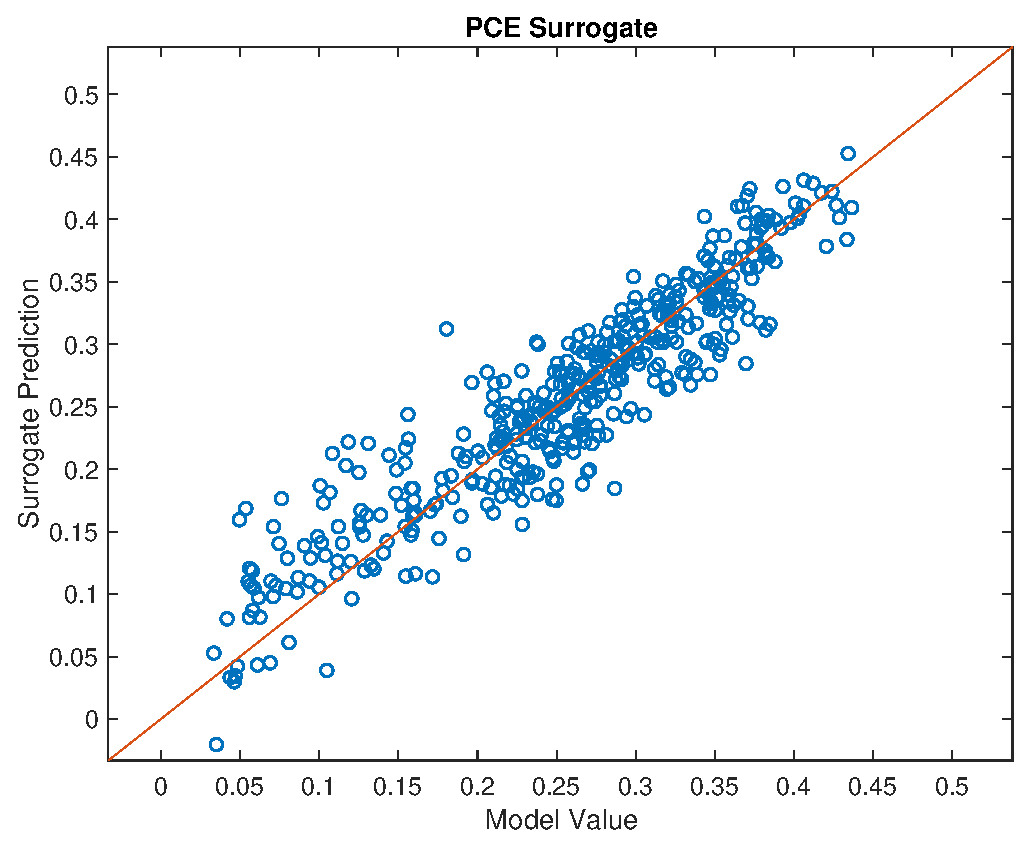
\includegraphics[width=.46 \textwidth]{Figures/AM_AMp_Min_QoI_PCE_Prediction_Experimental.eps}
\hspace{.1 cm}
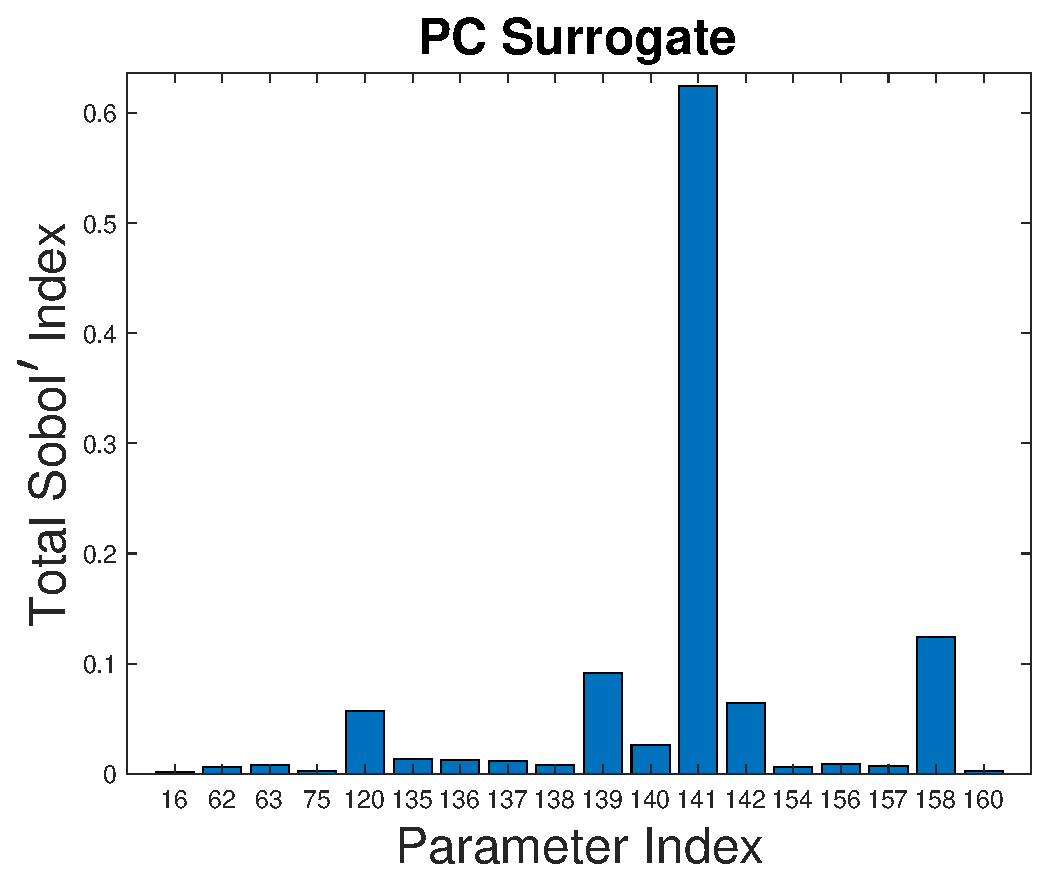
\includegraphics[width=.475 \textwidth]{Figures/AM_AMp_Min_QoI_PCE_SI_Experimental.eps}
\caption{$[AM+AM_p]_{min}$ QoI with experimental pulse stimulus. From left to right and top to bottom: linear surrogate predictions, linear surrogate importance measure, PC surrogate predictions, total Sobol' indices for PC surrogate.}
\label{fig:qoi_AM_AMp_Min_exp}
\end{figure}

The linear surrogate does not perform as well for this QoI; however, the PC surrogate is far more accurate; this highlights the nonlinearity of this particular QoI. 
%\todo[inline]{Tim: so why is this different to $\left( \frac{R}{R_o}\right) ^4$ when we have said that they are similar? Joey: They are sensitivity to a similar set of parameters, but they are two different functions. In particular, one QoI is constructed by integrating and the other by taking a minimum. This difference alone can change the complexity of approximating the function. Consider a simple example $f(x_1,x_2)=e^{x_1}+\epsilon x_2$ and $g(x_1,x_2)=x_1+\epsilon x_2$ for small $\epsilon$. It is clear that $f$ and $g$ are more sensitive to $x_1$ than $x_2$, but $f$ will be more difficult to approximate than $g$.}
 As in the previous results, parameter $\theta_{120}$ appears important in the linear surrogate and less important in the PC surrogate, albeit, it is more important for this QoI than the previous ones.

\begin{table}[h]
\centering
\ra{1.3}
\begin{tabular}{cccc}
\toprule
Parameter & Identification in Supplementary Material & Total Sobol' Index (exp.) & Total Sobol' Index (rect.) \\
\midrule
$\theta{141}$ & $z_4$ in equation (149)  & 0.6242 & 0.6203\\
$\theta{158}$ & $n_{cross}$ in equation (214)  & 0.1239 & 0.1488\\
$\theta{139}$ &  $z_2$ in equation (148)  & 0.0918 & 0.0954\\
$\theta{142}$ & $z_5$ in equation (149)  &0.0644 & 0.0629\\
$\theta{120}$ & Nominal value 5.5 in equation. (10)  & 0.0571 & 0.0240\\
 \arrayrulecolor{black}\bottomrule
\end{tabular}
\caption{Five most influential parameters for the $[AM+AM_p]_{min}$ QoI when the experimental pulse stimulus is applied. The leftmost column is the parameter, the left-center column identifies the parameter in the Supplementary Material, the right-center column is the total Sobol' index computed for the parameter using the experimental pulse stimulus, and the right column is the total Sobol' index computed for the parameter using the rectangular pulse stimulus.}
\label{tab:qoi_AM_AMp_Min}
\end{table}

%\section{Extra figures we probably won't include}
%\subsection{$AM_p$ Time Lag}
%
%\begin{figure}[h]
%\centering
%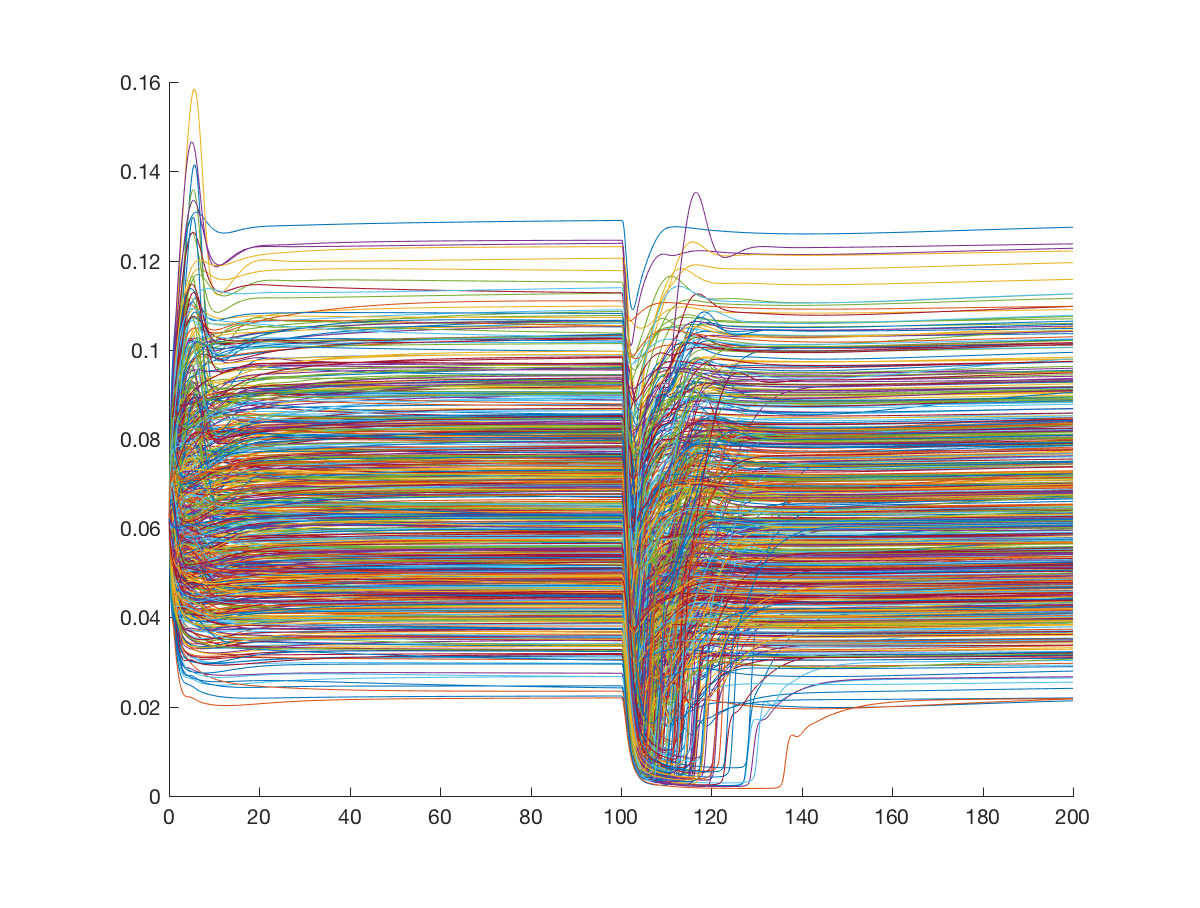
\includegraphics[width=.49 \textwidth]{Figures/AMp_Curves.eps}
%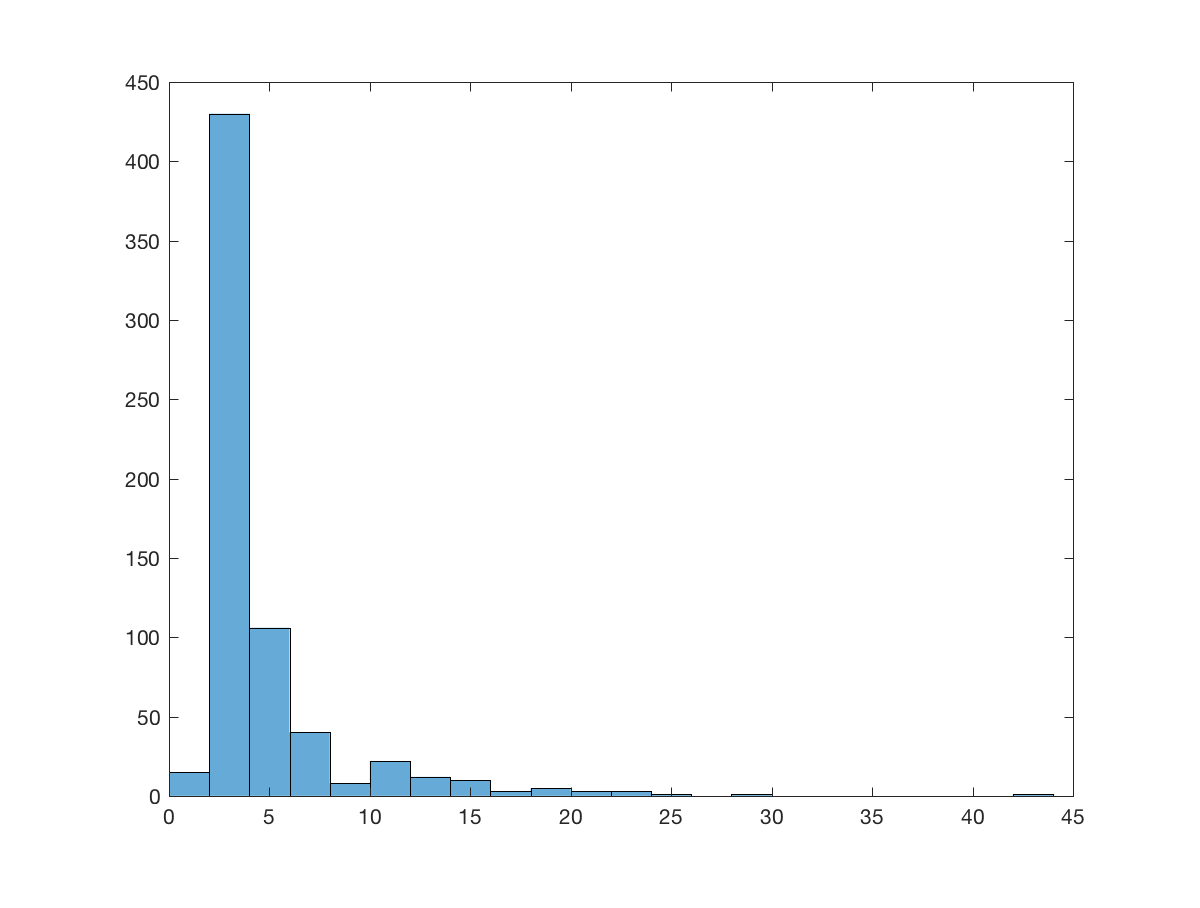
\includegraphics[width=.49 \textwidth]{Figures/AMp_Time_Lag_Histogram.eps}
%\caption{$AM_p$ curves on the left and a histogram of the time lags on the right.}
%\end{figure}
%
%\subsection{Radius Time Lag}
%
%\begin{figure}[h]
%\centering
%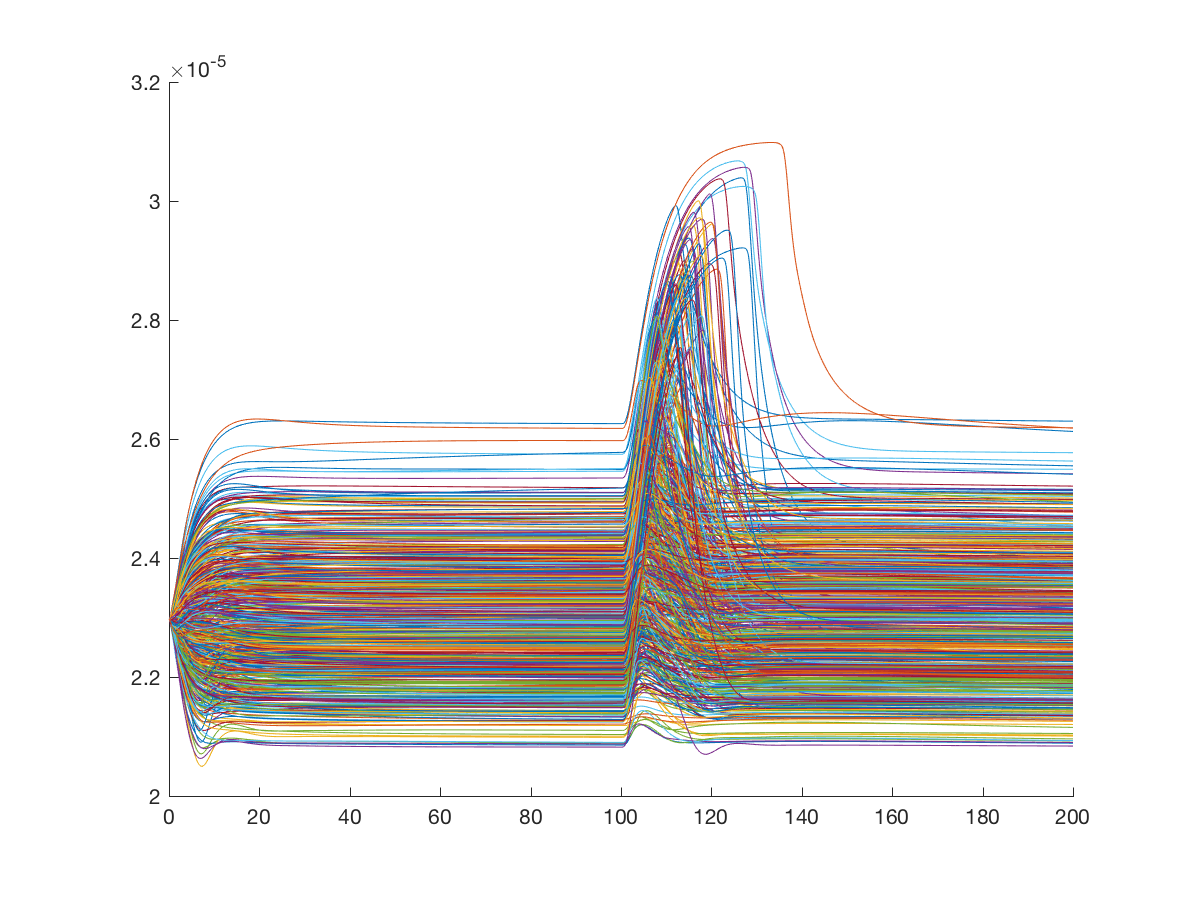
\includegraphics[width=.49 \textwidth]{Figures/Radius_Curves.eps}
%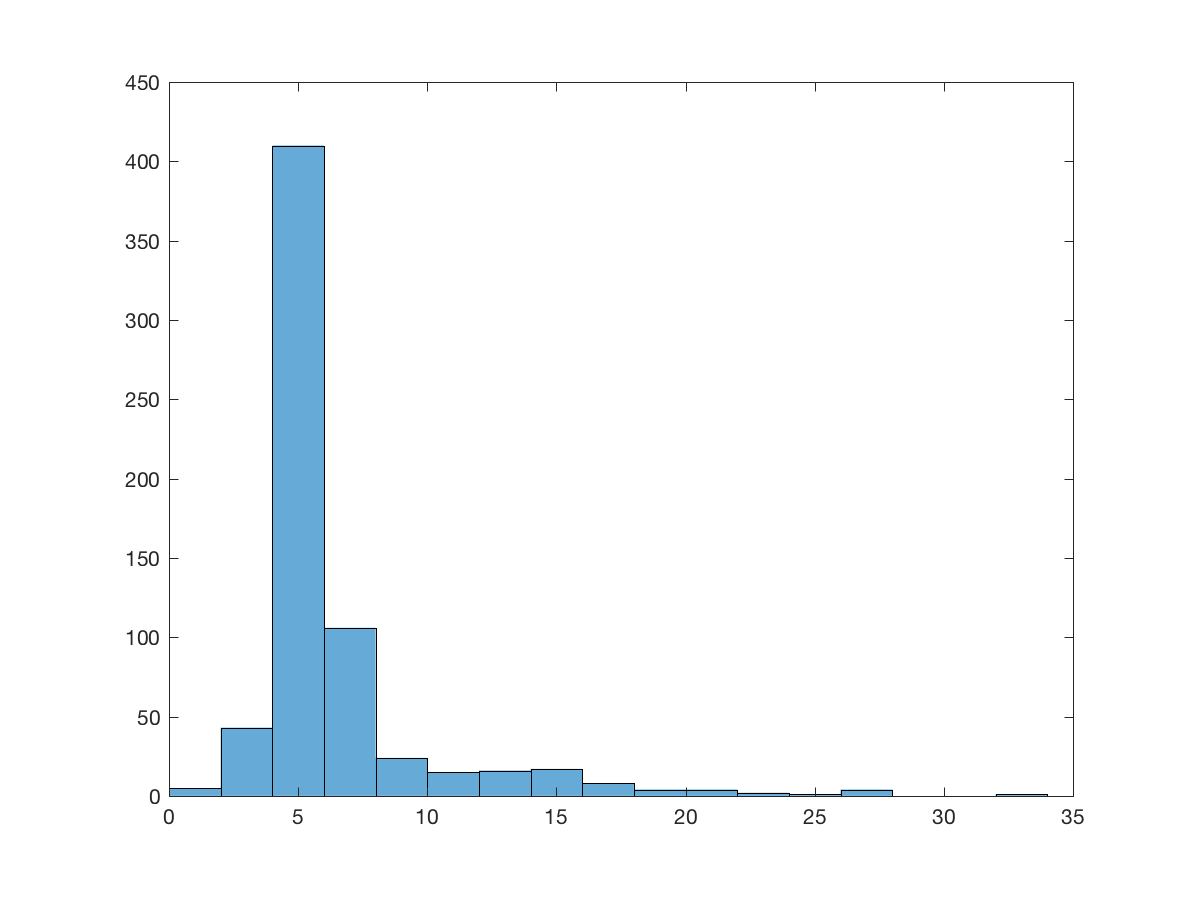
\includegraphics[width=.49 \textwidth]{Figures/Radius_Time_Lag_Histogram.eps}
%\caption{Radius curves on the left and a histogram of the time lags on the right.}
%\end{figure}
